\documentclass{article}

% if you need to pass options to natbib, use, e.g.:
\PassOptionsToPackage{numbers, compress}{natbib}
% before loading nips_2017
%
% to avoid loading the natbib package, add option nonatbib:
% \usepackage[nonatbib]{nips_2017}

\usepackage{nips_2017}

% to compile a camera-ready version, add the [final] option, e.g.:
% \usepackage[final]{nips_2017}

\usepackage[utf8]{inputenc} % allow utf-8 input
\usepackage[T1]{fontenc}    % use 8-bit T1 fonts
\usepackage{hyperref}       % hyperlinks
\usepackage{url}            % simple URL typesetting
\usepackage{booktabs}       % professional-quality tables
\usepackage{amsfonts}       % blackboard math symbols
\usepackage{nicefrac}       % compact symbols for 1/2, etc.
\usepackage{microtype}      % microtypography


%%%%%%%%%%%%%%%%%%%%%%%%%%%%%%%%%
% Custom packages
%%%%%%%%%%%%%%%%%%%%%%%%%%%%%%%%%
% AKM: already present above!
%\usepackage{hyperref}
\usepackage{amsmath}
\usepackage{amsfonts}
\usepackage{mathrsfs}
\usepackage{bm}
\usepackage{bbm}
\usepackage{stmaryrd}
\usepackage{algorithm}
\usepackage{algorithmic}
%\usepackage[sc]{mathpazo}
%\linespread{1.05}         % Palladio needs more leading (space between lines)
\usepackage[T1]{fontenc}    % use 8-bit T1 fonts
%\usepackage{subcaption}  % sub-figures
\usepackage{nicefrac}       % compact symbols for 1/2, etc.
\usepackage{microtype}      % microtypography
\usepackage{booktabs} % professional-quality tables
\usepackage{graphicx}
\graphicspath{{fig/}} % Location of the graphics files
\usepackage{pdfpages} % include multi-page PDF file

\usepackage{enumitem}

%%%%%%%%%%%%%%%%%%%%%%%%%%%%%%%%%
% Custom notation
%%%%%%%%%%%%%%%%%%%%%%%%%%%%%%%%%
\DeclareMathOperator*{\argmin}{argmin}
\DeclareMathOperator*{\argmax}{argmax}
\newcommand{\given}{\mid}
\newcommand{\llb}{\llbracket}
\newcommand{\rrb}{\rrbracket}
\newcommand{\indicator}[1]{\llbracket #1 \rrbracket}
\newcommand{\eat}[1]{}
\newcommand{\Q}{\mathsf{Q}}
\newcommand{\X}{\mathsf{X}}
\newcommand{\Y}{\mathsf{Y}}
\newcommand{\CCal}{\mathscr{C}}
\newcommand{\QCal}{\mathscr{Q}}
\newcommand{\XCal}{\mathscr{X}}
\newcommand{\YCal}{\mathscr{Y}}
\newcommand{\SSf}{\mathsf{S}}
\newcommand{\Real}{\mathbb{R}}
\newcommand{\E}[2]{\underset{#1}{\mathbb{E}}\left[ #2 \right]}
\newcommand{\ES}[2]{\underset{#1}{\mathbb{E}}\, #2}

% madeness: suPer-script in Brackets
\newcommand{\pb}[1]{^{({#1})}}

\newcommand{\bu}{\mathbf{u}}
\newcommand{\bv}{\mathbf{v}}
\newcommand{\bz}{\mathbf{z}}
\newcommand{\x}{\mathbf{x}}
\newcommand{\y}{\mathbf{y}}
\newcommand{\w}{\mathbf{w}}
\newcommand{\xii}{\mathbf{x}^{(i)}}
\newcommand{\yii}{\mathbf{y}^{(i)}}
\newcommand{\yij}{\mathbf{y}^{(ij)}}
\newcommand{\yik}{\mathbf{y}^{(ik)}}

\newcommand{\eg}{e.g.\ }
\newcommand{\ie}{i.e.\ }

\newcommand{\TODO}[1]{ {\color{blue}{\bf TODO:~{#1}}} }

% spacing black magic 
\newcommand{\secmoveup}{\vspace{-0.mm}}                %{\vspace{-0.12in}}
\newcommand{\ssecmoveup}{\vspace{-0.mm}}                %{\vspace{-0.12in}}
\newcommand{\bigsecmoveup}{\secmoveup\vspace{-0mm}}   %{\vspace{-0.08in}}
\newcommand{\textmoveup}{\vspace{-.0mm}}               %{\vspace{-0.08in}}
\newcommand{\bigtextmoveup}{\textmoveup\vspace{-0.0in}} %{\vspace{-0.06in}}
\newcommand{\itemmoveup}{\vspace{-0.mm}}                %{\vspace{-0.04in}}
\newcommand{\eqmoveup}{\vspace{-0.0in}}                 %{\vspace{-0.16in}}
\newcommand{\captionmoveup}{\eqmoveup\vspace{-0.0mm}}   %{\vspace{-0.16in}}
\newcommand{\refitemmoveup}{\vspace{-0.mm}}   			  %{\vspace{-0.16in}}


\title{Sequence Recommendation via Structured Prediction}

% The \author macro works with any number of authors. There are two
% commands used to separate the names and addresses of multiple
% authors: \And and \AND.
%
% Using \And between authors leaves it to LaTeX to determine where to
% break the lines. Using \AND forces a line break at that point. So,
% if LaTeX puts 3 of 4 authors names on the first line, and the last
% on the second line, try using \AND instead of \And before the third
% author name.

%%\author{
  %%David S.~Hippocampus\thanks{Use footnote for providing further
  %%  information about author (webpage, alternative
  %%  address)---\emph{not} for acknowledging funding agencies.} \\
  %%Department of Computer Science\\
  %%Cranberry-Lemon University\\
  %%Pittsburgh, PA 15213 \\
  %%\texttt{hippo@cs.cranberry-lemon.edu} \\
  %% examples of more authors
  %% \And
  %% Coauthor \\
  %% Affiliation \\
  %% Address \\
  %% \texttt{email} \\
  %% \AND
  %% Coauthor \\
  %% Affiliation \\
  %% Address \\
  %% \texttt{email} \\
  %% \And
  %% Coauthor \\
  %% Affiliation \\
  %% Address \\
  %% \texttt{email} \\
  %% \And
  %% Coauthor \\
  %% Affiliation \\
  %% Address \\
  %% \texttt{email} \\
%%}





\begin{document}
% \nipsfinalcopy is no longer used

\maketitle

\begin{abstract}
% !TEX root=./main.tex

%Playlists are a core feature of music streaming services.
Playlist recommendation concerns producing a sequence of songs that a user might enjoy.
We investigate this problem in three different cold-start scenarios:
%Specifically, we investigate three settings with different cold items:
(i) \emph{cold playlists}, where we recommend a set of songs to form a new playlist for an existing user; %without additional context except the user;
(ii) \emph{cold songs}, where we recommend newly released songs to extend existing playlists;
(iii) \emph{cold users}, where we recommend a set of songs to form a new playlist for a new user. %, without any other context.
%
We propose a flexible multitask learning method to deal with all three settings.
The method learns from user-curated playlists,
%the %multitask learning
%method
and encourages songs in the playlist 
to be ranked higher than those are not
by minimising a %the Bottom-Push
bipartite ranking loss.
We formulate the objective as a constrained convex optimisation problem,
and show how this may be approximated by an unconstrained objective
%then address the difficulty of a large number of constraints by approximating the %Bottom-Push loss
%bipartite ranking loss
%with a classification loss
inspired by an equivalence relationship between bipartite ranking and binary classification.
Empirical results on two real music playlist datasets show the proposed approach has good performance for playlist recommendation
in cold-start settings.
%in three cold-start settings.

\end{abstract}
\captionmoveup

%!TEX root = main.tex

\secmoveup
\section{Introduction}
\label{sec:intro}
\textmoveup

Content recommendation has been the subject of a rich body of literature~\citep{Goldberg:1992,Sarwar:2001,Koren:2010},
with established techniques seeing widespread adoption in industry~\citep{Linden:2003,Agarwal:2013,Amatriain:2015,Gomez-Uribe:2015}.
The success of these methods is explained by both the explosion in availability of user's explicit and implicit preferences for content,
as well as the design of methods that can suitably exploit these to make useful recommendations~\citep{Koren:2009}.

%LX: uh, 'unstructured' isn't a very well known way to refer to classic recsys
%For the most part, recommendation models have been limited to the case of static, \emph{unstructured} content.
Classical recommendation systems have focused on a fixed set of individual items such as movies, dubbed here as recommending \emph{unstructured} content.
While this setting has considerable value,
in many important scenarios one needs to recommend content that possesses some \emph{structure}.
%In its simplest form, this structure may be manifest by
%A wide-reaching
An example of this is where the desired content is naturally organized in
\emph{sequences} or {\em graphs}.
For example, consider %the problem of
recommending a trajectory of points of interest in a city to a visitor~\citep{lu2010photo2trip,lu2012personalized,ijcai15,cikm16paper}, a playlist of songs~\citep{McFee:2011,chen2012playlist,hidasi2015session,choi2016towards},
a chemical compound~\cite{dehaspe1998finding} or a few linked websites for e-commerce~\cite{antikacioglu2015recommendation}.
%
%a playlist of songs to users based on their listening history~\citep{McFee:2011,chen2012playlist,hidasi2015session,choi2016towards}.
%LX - do we want to broaden the definition and down-play music playlist?

A na\"{i}ve approach to sequence recommendation is to ignore the structure.
%and learn a standard recommendation model.
% In the playlist example, we could learn a user's preference for individual songs,
% and then create a playlist based on the top ranked songs.
In the trajectory example, we could learn a user's preference for individual locations,
and create a trajectory based on the top ranked locations.
However, such an approach may be sub-optimal:
%This however completely ignores the fact that while a user's
for example,
in the trajectory recommendation problem, it is unlikely a user will want to visit three restaurants in a row.
Similarly,
while a user's two favourite songs might belong
the metal and country genres respectively,
it is questionable that a playlist featuring these songs in succession will be as enjoyable to the user.

The above raises the question of how one can effectively learn from such sequential content.
In this paper, we show how to cast sequence recommendation as a \emph{structured prediction} problem,
which allows us to leverage the toolkit of structured SVMs~\citep{tsochantaridis2005large}.
However, a vanilla application of such methods does not suffice,
as they do not account for the fact that each input can have multiple ground truths,
and that repeated elements in predicted sequences are undesirable.
We show how to overcome this by
incorporating multiple correct sequences into a structured prediction formulation,
%suitably normalising the loss function for the model,
%LX - what's the right word here?  i feel normalising is only summarizing part of what is done??
and by two novel applications of the list Viterbi algorithm that sequentially finds the list of top-scoring sequences.
%LX - marketing listViterbi
%modifying the inference and prediction steps using a variant of the Viterbi algorithm.
Specifically, our contributions are as follows:
\begin{itemize}[noitemsep,leftmargin=12pt]\itemmoveup
	\item We formalise the problem of sequence recommendation (\S\ref{sec:seqrec-defn}), and show how trajectory recommendation can be seen as a special case (\S\ref{sec:trajrec}).
	%cast it as a structured prediction task (\S\ref{sec:recseq}), and .

	\item We show how sequence recommendation may be attacked using structured SVMs (\S\ref{sec:recseq}).
	We propose one improvement of structured SVMs to the recommendation problem, so as to account for the existence of multiple ground truths for each input (\S\ref{ssec:sr}).
	%Following \citep{joachims2009cutting}, we propose both $n$-slack and 1-slack versions of the structured recommender.%\footnote{This new structured recommender can in principle be applied to any problem where loss augmented inference can be efficiently computed. We focus on sequence recommendation in this paper.}

    \item We propose two novel applications of the list Viterbi algorithm -- an extension of the classic Viterbi algorithm that sequentially finds the list of highest scored sequences under some model --
to exclude multiple ground truths for model learning (\S\ref{ssec:training}),
and to predict sequences without repeated elements, i.e. {\em path}s in state-space (\S\ref{ssec:testing}).
	%\item We show how one can avoid recommending sequences with loops or repetitions via integer linear programming and list Viterbi;
%an extension of the classic Viterbi algorithm that returns a list of the highest scored sequences under some model;
%%	We show that these algorithms may be incorporated during both the training %(via loss augmented inference)
%%	and prediction steps of our structured recommendation (\S\ref{ssec:training}, \S\ref{ssec:testing}).
	%LX - now we have only four bullet points, i'm happier with this -- 5 is too many!
	%LX - in addition, i do not think we can claim ILP as a contribution. it's in Lim'2015

	\item We present experiments on real-world trajectory recommendation problems, and demonstrate our structured recommendation approaches improve over existing non-structured baselines (\S\ref{sec:experiment}).\itemmoveup
\end{itemize}

%We begin with an overview of related work, before presenting our model.
%We begin with an overview of the sequence recommendation problem, before presenting our model.


%!TEX root = main.tex
%\secmoveup
\section{A structured prediction approach to sequence recommendation}
%\section{Sequence recommendation via structured prediction}
\label{sec:recseq}
%\textmoveup

We now describe a method to
solve sequence recommendation problems, such as trajectory recommendation.
We first provide background on structured SVMs, % (Sec~\ref{ssec:ssvm}),
then present a model for structured recommendation, % (Sec~\ref{ssec:sr}),
followed by the correspondingly updated algorithms for its learning % (Sec~\ref{ssec:training})
and inference. % (Sec~\ref{ssec:testing}).


%\secmoveup
\subsection{Background: SSVM for structured prediction}
\label{ssec:ssvm}
%\textmoveup

Recall that structured prediction involves predicting a structured label $\y \in \mathcal{Y}$ for an input $\x \in \mathcal{X}$,
via a score function $f(\x,\y)$.
%A popular model is the Structured Support Vector Machine (SSVM)~\cite{taskar2004max,tsochantaridis2004support}, comprising three core ingredients.
A popular approach is the Structured Support Vector Machine (SSVM)~\cite{taskar2004max,tsochantaridis2004support}, 
comprising three key ingredients.

\subsubsection{Score function}
In SSVMs, %we specify that 
the score function $f(\x, \y)$ takes a linear form, \ie
$f(\x, \y) = \w^\top \Psi(\x, \y)$,
where $\w$ is a weight vector, and $\Psi(\x, \y)$ is a \emph{joint feature map}.
The design of the feature map $\Psi$ is problem specific.
For sequence prediction problems,
%%where $\y = y_{1 : l}$
%For many problems,
%we may assume that it
%%a popular choice
%%is a vector whose elements represent
one may
consider the unary
terms for each element in the label $y_{1:l}$, and pairwise interactions between
adjacent elements in the label,
%For sequence data, %in particular,
%we also
% We may further
% assume that the pairwise interactions are between
% adjacent elements,
i.e. $y_j$ and $y_{j+1}$ for $j=1 \! : \! l \!-\! 1$.
Subsequently, $f(\x,\y)$ decomposes into a weighted sum of
each of these features: %with the corresponding feature weight:
\begin{equation}
\label{eq:jointfeature}
\resizebox{0.909\linewidth}{!}{$\displaystyle
f(\x, \y) = %\w^\top \Psi(\x, \y) =
\sum_{j=1}^l \w_j^\top \psi_j(\x, y_j) + \sum_{j=1}^{l-1} \w_{j,j+1}^\top \psi_{j,j+1}(\x, y_{j}, y_{j+1}).
$}
%\eqmoveup
\end{equation}
Here, $\psi_j$ is a feature map between the input and one output label element $y_j$, with a corresponding weight vector $\w_j$,
and $\psi_{j,j+1}$ is a pairwise feature vector that captures the interactions between consecutive labels $y_j$ and $y_{j+1}$,
with a corresponding weight vector $\w_{j,j+1}$.

%To learn the parameters, we train the structured SVM by optimising a quadratic program (QP),
\subsubsection{Objective function}
To learn a suitable weight vector $\w$ from input $\{\x\pb{i}, \y\pb{i}\}_{i=1}^n$,
SSVMs solve: %the following optimisation problem:
\begin{equation}
\label{eq:nslack}
\resizebox{0.909\linewidth}{!}{$\displaystyle
\begin{aligned}
& \min_{\w, \, \bm{\xi} \ge 0} \ \frac{1}{2} \w^\top \w + \frac{C}{n} \sum_{i=1}^n \xi_i, 
\ s.t. \ \forall i, \\
& \ \w^\top \Psi(\x^{(i)}, \y^{(i)}) - \w^\top \Psi(\x^{(i)}, \bar{\y}) \ge
  \Delta(\y^{(i)}, \bar{\y}) - \xi_i, \, \forall \bar\y \in \mathcal{Y}.
\end{aligned}
$} %\eqmoveup
\end{equation}

Here,
$\mathcal{Y}$ is the set of all possible sequences,
$\Delta(\y\pb{i}, \bar\y)$ is the loss function between $\bar\y$ and the ground truth $\y\pb{i}$,
and slack variable $\xi_i$ is the \emph{hinge loss} for the prediction of the $i$-th example. %~\cite{tsochantaridis2004support}.
Alternatively, we can use \emph{one} slack variable to represent the sum of the $n$ hinge losses in~(\ref{eq:nslack}),
\ie the 1-slack formulation~\cite{joachims2009predicting}.
%%To solve problem (\ref{eq:nslack}),
% one option is to simply enumerate all constraints, and feed the problem into a standard solver.
% However, this approach is impractical as there is a constraint for every possible label $\bar{\y}$.
%recently developed learning schemes such as
%%cutting-plane algorithms~\cite{joachims2009predicting}, % cutting-plane
%%gradient-based algorithms~\cite{ratliff2006subgradient} % sub-gradient
%%and conditional gradient methods~\cite{lacoste2013block} % Frank-Wolfe
%can efficiently optimise the objective and
%%are widely used in practice~\cite{muller2014methods}.
%LX - do we want to say the gradient-based methods are inefficient??
%Instead, we can resort to a cutting-plane algorithm which repeatedly solves the quadratic program (\ref{eq:nslack})
%with a growing set of constraints~\cite{joachims2009predicting}.
%In each iteration, a new constraint is formed by solving the loss-augmented inference,
%which helps shrink the feasible region of the problem.


\subsubsection{Loss-augmented inference}
We can rewrite the constraints in (\ref{eq:nslack}) as
$\max_{\bar\y \in \mathcal{Y}} \left\{ \Delta(\y\pb{i}, \bar\y) + \w^\top \Psi(\x\pb{i}, \bar\y) \right\} \le
\w^\top \Psi(\x\pb{i}, \y\pb{i}) + \xi_i$.
The maximisation at the left side is known as \emph{loss-augmented inference}.
%refers to the inner maximisation in Eq.~(\ref{eq:hingeloss}).
%This formulation is called "$n$-slack" as we have one slack variable for each example in training set.
%Here the inner maximisation is known as the \emph{loss-augmented inference}.
When the underlying graph of SSVM is a tree (which is the case for sequence recommendation),
this inference may be solved efficiently if the loss function $\Delta(\cdot,\cdot)$ is decomposable
with respect to individual and pairs of label elements,
\eg using the Viterbi algorithm~\cite{joachims2009predicting}.
% in a way similar to Equation~\eqref{eq:jointfeature}.

%\secmoveup
%\subsection{SSVM for structured recommendation: the SP and SR models}
\subsection{SSVM for sequence recommendation}
\label{ssec:sr}
%\textmoveup

We now present two possible means of applying SSVMs to sequence recommendation.

\subsubsection{The SP model}
Recall that sequence recommendation
involves observing \emph{multiple} ground truth outputs for each input, \ie
%If we observed more than one labels for a particular set of features,
%The classic SSVM described in Section~\ref{ssec:ssvm} can be generalised to capture this setting:
for input $\x\pb{i}$, there is a set of ground truths $\{\y\pb{ij}\}_{j=1}^{n_i}$.
%where $n_i$ is the number of labels for $\x^{(i)}$.
% describe duplicating examples
One na\"{i}ve approach to the problem
is creating
$n_i$ examples $\{(\x\pb{i}, \y\pb{ij})\}_{j=1}^{n_i}$,
and feeding this to the classic SSVM. %described in Section~\ref{ssec:ssvm} to capture this setting
We call this the \emph{structured prediction} (\emph{SP}) model.
%
The SP model is appealing due to its simplicity.
However, it is sub-optimal:
%The problem with this approach is in the result of loss-augmented inference,
%\ie
%%
%% DW: no need to exclude \yik
%%the result of loss-augmented inference on $(\xii, \yij)$ could be any label $\yik \in \{\yij\}_{j=1}^{n_i} \setminus \{\yij\}$,
%%but then we would incorrectly penalise predicting $\yik$ for $\xii$.
%%
the result of loss-augmented inference on $(\x\pb{i}, \y\pb{ij})$ could be a ground truth label $\y' \in \{\y\pb{ij}\}_{j=1}^{n_i}$,
which means we would incorrectly penalise predicting $\y'$ for $\x\pb{i}$.

\subsubsection{The SR model}
To overcome the limitation of the SP model,
we propose the following \emph{structured recommendation} (\emph{SR}) model that extends the SSVM to explicitly incorporate multiple ground truths: %for each example.
%We can learn an \emph{SR} model by optimising %a quadratic program similar to (\ref{eq:nslack}),
\begin{equation}
\label{eq:nslack_ml}
\resizebox{0.909\linewidth}{!}{$
\begin{aligned}
& \min_{\w, \, \bm{\xi} \ge 0} \ \frac{1}{2} \w^\top \w + \frac{C}{N} \sum_{i=1}^n \sum_{j=1}^{n_i} \xi_{ij},
\ s.t. \ \forall i, \, \forall j, \\
& \ \w^\top \Psi(\x^{(i)}, \y^{(ij)}) - \w^\top \Psi(\x^{(i)}, \bar{\y}^{(i)}) \ge
  \Delta(\y^{(ij)}, \bar{\y}^{(i)}) - \xi_{ij}.
\end{aligned}
$}
\end{equation}
where $N = \sum_i n_i$ and $\bar{\y}^{(i)} \in \mathcal{Y} \setminus \{\y^{(ij)}\}_{j=1}^{n_i}$.
The 1-slack formulation of~(\ref{eq:nslack_ml}) can be formed similar to that of~(\ref{eq:nslack}).
Intuitively, the objective in (\ref{eq:nslack_ml}) is similar to a ranking objective, as the constraints enforce
that the positively labeled sequences 
%(the known items that the user likes) 
(items that the user likes) 
are scored higher than all other unseen sequences.
Such objectives have been proven useful in classic unstructured recommendation~\cite{bpr09}.
%Recent work on positive and unlabelled data have
%theoretically shown the close relationship between positive and unlabelled learning and two class classification.

Compared to the SP model (\ref{eq:nslack}), the key distinction is that (\ref{eq:nslack_ml})
explicitly \emph{aggregates} all the ground truth sequences for each input when generating the constraints,
\ie the loss-augmented inference becomes
\begin{equation}
\label{eq:loss_aug_inf}
\resizebox{0.909\linewidth}{!}{$
%\max_{\bar{\y}^{(i)} \in \ \mathcal{Y} \setminus \{\y^{(ij)}\}_{j=1}^{n_i}}
\underset{\bar{\y}^{(i)} \in \ \mathcal{Y} \setminus \{\y^{(ij)}\}_{j=1}^{n_i}}{\max}
     \left( \Delta(\y^{(ij)}, \bar{\y}^{(i)}) + \w^\top \Psi(\x^{(i)}, \bar\y^{(i)}) \right).
$}
\end{equation}
In this way, we do not have contradictory constraints where
two ground truth sequences are each required to have larger score than the other.

%%As a remark, we note that instead of using $N$ slack variables as that in (\ref{eq:nslack_ml}),
%%we can use \emph{one} slack variable to represent the sum of the $N$ hinge losses. % in (\ref{eq:nslack_ml}).
%which leads to a $1$-slack formulation
%This $1$-slack formulation can be learned more efficiently than the $N$-slack formulation (\ref{eq:nslack_ml}) if training using cutting-plane algorithm.
%%This 1-slack formulation (see supplement) can be learned more efficiently than (\ref{eq:nslack_ml})
%%when training using cutting-plane algorithms. %the above can be learned more efficiently than (\ref{eq:nslack_ml}).

The SP and SR models can be learned using a rich set of training schemes such as
cutting-plane algorithms~\cite{joachims2009predicting}, % cutting-plane
gradient-based algorithms~\cite{ratliff2006subgradient} % sub-gradient
and conditional gradient methods~\cite{lacoste2013block}, % Frank-Wolfe
given proper loss augmented inference and prediction procedures,
which we describe subsequently. %in the next two sections.

%DW: do we need this paragraph?
%LX - the sentence below contains little info
%To describe how to use the above models for sequence recommendation, we must precisely describe how one performs training and prediction using them.
Beyond dealing with multiple ground truths,
one additional requirement is for the predicted sequence to be a {\em path}.
This is a {\em global} constraint bringing new challenges for prediction and loss-augmented inference.
%that makes the underlying graph structure no longer a tree,
The following two sections describe the training and prediction with these requirements.
%This is the focus of the next two sections.

\subsection{SP and SR model training}
\label{ssec:training}

The main challenge in training the SP and SR models is performing loss-augmented inference~(\ref{eq:loss_aug_inf}).
As noted above, the SP model can be trained as per the vanilla SSVM.
The SR model, however, requires modifying the training procedure to account for the existence of multiple ground truths.
In particular, (\ref{eq:loss_aug_inf}) needs to be solved by \emph{excluding the sequences} $\{\y\pb{ij}\}_{j=1}^{n_i}$, and ideally with {\sc path} constraints.
We show in the following how to address both problems with an extension of the Viterbi algorithm.

%% DW: do we need to describe this here?
%%
%%For both models, a further, subtler desiderata is to
%%\emph{avoid sequences that have loops} in loss-augmented inference.
%%The motivation is that, as mentioned in \S\ref{sec:trajrec}, repeated elements are often undesirable in sequence recommendation
%%\eg a user will likely not want to visit the same location twice.


\subsubsection{List Viterbi algorithms}
List Viterbi represents a family of algorithms originally invented to decode digital signals corrupted by noise~\cite{seshadri1994list}, or to find more than one candidate sentence in speech recognition~\cite{soong1991tree}. Given a score function that can be decomposed into unary and pairwise costs such as (\ref{eq:jointfeature}), a list Viterbi algorithm finds the $k$ highest scoring sequences. % that has the highest score.
\eat{%% removed to shorten the narrative
The \emph{parallel list Viterbi} algorithm~\cite{seshadri1994list} finds the top $k$ sequences
by keeping $k$ backtrack pointers for each possible state in each position of the sequence.
This algorithm is memory-inefficient and can be difficult to use when $k$ is unknown \emph{a-priori} %one does not know what $k$ to use apriori 
-- this is the case for both the learning and inference challenges in this work.
}

A particularly applicable variant is the \emph{serial list Viterbi} algorithms (SLVA)~\cite{seshadri1994list,nilsson2001sequentially}, when the number of sequences to find is unknown a priori. 
This algorithm sequentially find the $k$-th best sequences given the best, 2nd best, \dots, $(k \!-\! 1)$-th best sequences.
%The key insight here is 
\citet{seshadri1994list} observed 
that the 2nd best sequence deviates from the best sequence
for one continuous segment, and then merges back to the best sequence without deviating again
-- otherwise replacing one of the continuous segments with those from the best sequence will increase the score.
Subsequently, the $k$th best sequence can be the 2nd best sequence relative to the $(k \!-\! 1)$-th best sequence
at the point of final merge, or the 2nd or 3rd best sequence to the $(k \!-\! 2)$-th best sequence at the point of final merge, \ldots, and so on. 
\citet{nilsson2001sequentially} observed that the same goal can be achieved by cleverly partitioning the search space into subsets of sequences that share a prefix with the current list of best sequences. While derived in different communities, it is not hard to show that these two algorithms are in fact fundamentally identical.
%SLVA works by keeping track of the score differences to the best sequences and merge points along the sequences. 
See supplement for a complete description.

We use SLVA in two different ways, first to deal with multiple ground truths, and second to find paths.


\subsubsection{Eliminating multiple ground truths}
Recall that standard loss-augmented inference for an SSVM (for sequences) may be done with the classic Viterbi algorithm, but the best-scoring sequence could be in the ground-truth set $\{\y^{(ij)}\}_{j=1}^{n_i}$. We check whether this is the case, and if it is, use SLVA to decode the next best sequence until we find one that is not in the ground truth set.
%The serial list Viterbi allows exclusion of sequences with repeats,
%as well as
%excluding an arbitrary number of known sequences.
%The list Viterbi algorithm is fully detailed in the supplement.
Note that the serial list Viterbi algorithm
can be used for loss-augmented inference with Hamming loss, the most common loss function for sequence prediction tasks,
since it only requires the loss function be decomposable with respect to the label elements.


\subsubsection{Eliminating loops: \textsc{SPpath} and \textsc{SRpath}}
%Having seen the viability of the list Viterbi algorithm for removing known sequences from consideration during inference,
The list Viterbi algorithm can also enforce that loss-augmented inference only considers sequences that are \emph{paths}. This may be done by checking if each of the next-best sequences has a loop, and following SLVA as above.
This idea can be applied to both the SP and SR models, as enforcing path constraints is independent of excluding multiple ground truths.
We call the resulting models \textsc{SPpath} and \textsc{SRpath} respectively.

%LX - remark, doesn't have to be here. intuition for the real extension to SLVA?
Note that $k$ is expected to be small in noisy signal recovery, such as digital communications~\cite{seshadri1994list} and speech recognition~\cite{soong1991tree}. But this is not necessarily the case for inference in SR models.

%\secmoveup
\subsection{SP and SR model prediction}
\label{ssec:testing}
%\textmoveup

For both the SP and SR models, prediction requires that we compute $\argmax_{\y \in \mathcal{Y}_{\mathrm{path}}} f( \x, \y )$.
This is the maximum over $\mathcal{Y}_{\mathrm{path}} \subseteq \mathcal{Y}$,
which comprises all elements of $\mathcal{Y}$ that are paths. % and not all possible sequences.


\subsubsection{Eliminating loops: SLVA and ILP}
Observing that the prediction requires excluding a set of sequences from consideration, a natural and effective idea is to once again apply the {list Viterbi algorithm} of the previous section.

Alternately, we observe that our {\em path-decoding} problem is a variant of the well-known
{\em traveling salesman problem} (TSP), in particular the best of ${m \choose l}$ TSPs, 
where $m$ denotes the total number of points.
%LX - uh, do we need to explain, or is this obvious
This is because list Viterbi keeps searching the next best sequence %can find all best-scoring sequences 
until a path is discovered, %one of which is a path, 
while TSP can be formulated to find the best path.
This equivalence opens new possibilities to leverage well-studied TSP formulations
and modern implementations~\cite{tspbook2011}. In particular, we consider an integer linear program (ILP) formulation of the TSP (Eq.~\ref{eq:obj} to \ref{eq:cons4}). This formulation extends earlier work on sequence recommendation~\cite{lian2014geomf,cikm16paper} by systematically incorporating unary and pairwise scoring terms.
%LX - is the last sentence true?

%LX -- getting rid of this prelim redundant discussion
%LX - also moving Christofeds to the end of the section
%Consider the setting of finding the best path $\y^*$ that starts from a specific point $y_1^*$ and traverses exactly $l$ of $m$ candidate points.
%Given desired sequence length $l$ among $m$ possible points, the Viterbi algorithm~\cite{tsochantaridis2005large}
%will generate the length-$l$ sequence $\y^*$ with the best score. %i.e. $\y^* = \argmax_\y f(\x,\y)$.

%LX - this paragraph is logically confusing, restructure
%Such a point traversal problem can be solved by incorporating
%sub-tour elimination constraints of the TSP~\cite{ijcai15,cikm16paper}.
%In particular, %%the integer linear program (ILP) formulation (Eq.~\ref{eq:obj} to \ref{eq:cons4})
%%will solve SR inference for path $\y^*$ of length $l$ by decoding an optimal solution.
%it can be solved by decoding an optimal solution of the integer linear program (ILP) Eq.~\ref{eq:obj} to \ref{eq:cons4}.

Given a set of points $\{p_j\}_{j=1}^m$,
consider binary variables $u_{jk}$ that are true iff
the transition from $p_j$ to $p_k$ is in the resulting path,
and binary variables $z_j$ that are true iff
the optimal path $\y^*$ terminates at $p_j$.
%$p_j$ is the last point in $\y^*$.
%Suppose that $l$ is the number of candidate POIs.
For brevity, we index the points such that $y_1^* = p_1$.
Firstly, the desired path should start from $y_1^*$ (Eq.~\ref{eq:cons1}).
In addition, only $l\!-\!1$ transitions between points are permitted as the path length is $l$ (Eq.~\ref{eq:cons2}).
Moreover, any point could be visited at most once (Eq.~\ref{eq:cons3}).
The last constraint, where $v_j \in \mathbf{Z}$ is an auxiliary variable,
%enforces that $\y^*$ is a single sequence of points without sub-tours.
ensures $\y^*$ does not have disjoint cycles~\cite{Miller:1960}.
%\TODO{LX: i do not understand the last contraint, $v_j$ did not seem to have been defined? are they binary or something else?}
% DW: v_j defined in the first constraint, which is a natural number
We rewrite Eq.~(\ref{eq:jointfeature}) into a linear function of variables $u_{jk}$
(dropping the constant unary term for $y_1^*$), as % which results 
in~(\ref{eq:obj}).
%\setlength{\belowdisplayskip}{1pt} \setlength{\belowdisplayshortskip}{0pt}
%\setlength{\abovedisplayskip}{1pt} \setlength{\abovedisplayshortskip}{0pt}
%\begin{equation}%\eqmoveup\eqmoveup
%\label{eq:obj}
%\max_{\bu} ~\sum_{k=1}^m \w_k^\top \psi_k(\x, p_k) \sum_{j=1}^m u_{jk} +
%            \sum_{j,k=1}^m u_{jk} \w_{jk}^\top \psi_{j, k}(\x, p_j, p_k)
%\end{equation}
%{$\displaystyle
%\begin{minipage}{0.45\linewidth}
%\begin{alignat}{2}
%s.t. \,
%& \sum_{k=2}^m u_{1k} = 1, \, \sum_{j=2}^m u_{j1} = z_1=0                 \label{eq:cons1} \\
%& \sum_{j=1}^m \sum_{k=1}^m u_{jk} = l-1, \, \sum_{j=1}^m u_{jj}=0        \label{eq:cons2}
%\end{alignat}
%\end{minipage}
%\qquad
%\begin{minipage}{0.5\linewidth}
%\begin{alignat}{3}
%\sum_{j=1}^m u_{ji} = z_i &+ \sum_{k=2}^m u_{ik} \le 1, \, i = 2,\cdots,m  \label{eq:cons3} \\
%v_j - v_k + 1 &\le (m-1) (1-u_{jk}),                                       \nonumber \\
%              & \qquad j,k = 2,\cdots,m                                    \label{eq:cons4}
%\end{alignat}
%\end{minipage}
%$}
\vspace{-.4em}
\begin{equation}
\label{eq:obj}
\resizebox{0.909\linewidth}{!}{$\displaystyle
\max_{\bu} ~\sum_{k=1}^m \w_k^\top \psi_k(\x, p_k) \sum_{j=1}^m u_{jk} +
            \sum_{j,k=1}^m u_{jk} \w_{jk}^\top \psi_{j, k}(\x, p_j, p_k)
$}
\end{equation}
%
\begin{small}
\vspace{-1.2em}
\begin{align}
s.t. \, 
& \sum_{k=2}^m u_{1k} = 1, \, \sum_{j=2}^m u_{j1} = z_1=0                   \label{eq:cons1} \\
& \sum_{j=1}^m \sum_{k=1}^m u_{jk} = l-1, \, \sum_{j=1}^m u_{jj}=0          \label{eq:cons2} \\
& \sum_{j=1}^m u_{ji} = z_i + \sum_{k=2}^m u_{ik} \le 1, \, i = 2,\cdots,m  \label{eq:cons3} \\
& v_j - v_k + 1 \le (m-1) (1-u_{jk}), \, j,k = 2,\cdots,m                   \label{eq:cons4}
\end{align}
\end{small}

\vspace{-1.3em}

\subsubsection{Recommending more than one trajectory}
Since multiple possible trajectories can start at the same POI, 
It is desirable %we need 
to predict multiple trajectories for a query. %each test query. 
% ILP for top-k prediction/inference
%\textbf{Top-$K$ prediction}.
We can use the above ILP formulation to find the top-$K$ scored paths in a sequential manner.
In particular, given the $K\!-\!1$ top scored paths $\{\y\pb{k}\}_{k=1}^{K-1}$,
the $K\!$-th best scored path can be found by solving the above ILP with additional constraints:
%%\begin{equation}
%%\label{eq:topk_ILP}
$\sum_{j=1}^{l-1} u_{y_j, y_{j+1}} \le l-2, ~\forall \y \in \{\y^{(k)}\}_{k=1}^{K-1}$.
%%\end{equation}
Alternatively, we can achieve this by %using 
the same approach as when eliminating ground truth sequences using SLVA.


% ILP for learning (loss-augmented inference)
\subsubsection{Eliminating multiple ground truths with ILP?}
A natural question is whether one can use the above ILP
to exclude observed labels when training an SR model,
\ie solving the loss-augmented inference~(\ref{eq:loss_aug_inf}).
In fact, this may be done
%together with constraints~(\ref{eq:cons1})-(\ref{eq:cons4}),
as long as the loss $\Delta(\y,\bar\y)$ can be represented as a linear function of $u_{jk}$.
One example is the number of mis-predicted POIs disregarding the order $\Delta(\y, \bar\y) = \sum_{j=2}^l (1 - \sum_{k=1}^m u_{k, y_j})$.
However, we note that Hamming loss %%, the most common loss function for sequence prediction tasks,
%cannot be used here, 
is not applicable here,
as $\Delta(\y,\bar\y) = \sum_{j=1}^l (1 - \llb y_j = \bar y_j \rrb)$
cannot be expressed as a linear function of $u_{jk}$.


\subsubsection{Practical choices: ILP vs SLVA vs other heuristics}
When performing prediction for SP and SR model, we found that state-of-the-art ILP solvers converge to a solution faster
than the serial list Viterbi algorithm if the sequence length $l$ is large.
The reason is, while list Viterbi algorithms are polynomial time given the list depth $k$~\cite{nilsson2001sequentially},
in reality $k$ is unknown a priori and can be very large for long sequences.
We therefore use ILP for very long ($l\ge10$) sequences in the experiments (otherwise the list Viterbi algorithm is applied).

One might also consider the well-known Christofides algorithm~\cite{christofides1976} to eliminate loops in a sequence, as this is known to generate a solutions within a factor of 3/2 of the optimal solution for traveling salesman problems. However, the resulting sequence will have less than the desired number of points, and the resulting score will not be optimal.


\subsection{Discussion}
The unary terms in the sequence scoring function \eqref{eq:jointfeature} can be replaced with {\em personalised} terms to each user, such as from a recommender system~\cite{Koren:2009,bpr09}. 
We also note that the sequence recommendation problem suits recurrent neural networks (RNNs) based techniques.
However, these techniques generally require much more training data than available in our problem.
It is also not clear how to recommend a sequence as a whole instead of recommending the next best location as proposed in recent RNNs based work~\cite{aaai16}.
We leave this and personalising sequence recommendation as future work.


% \subsection{SSVM for sequence recommendation: sequence decoding}
% \label{ssec:subtour}
% \label{ssec:SRinf}

% The SR model require two algorithmic components for inference and learning
% (missing from the SSVM algorithms).
% For inference, SR needs to predict a {\em path}, \ie a sequence whose elements are distinct from each other,
% that maximises the score function (Eq.~\ref{eq:jointfeature}).
% As described in Section~\ref{sec:intro}, this is desirable since users traversing a sequence (of locations or music)
% would not want to see repeated entries.
% Given desired sequence length $l$ among $m$ possible points, the Viterbi algorithm~\cite{tsochantaridis2005large}
% will generate the length-$l$ sequence $\y^*$ with the best score. %i.e. $\y^* = \argmax_\y f(\x,\y)$.
% One may then use the well-known
% Christofides algorithm~\cite{christofides1976} on $\y^*$ to eliminate loops in the sequence.
% However, the resulting sequence will have less than the desired number of points, and the resulting score will not be optimal in general.

% For learning an SR model, loss-augmented inference (\ref{eq:loss_aug_inf}) needs to be done by excluding multiple known sequences.
% As described in Section~\ref{ssec:sr}, %this involves %we would want to maximize the loss-augmented objective function
% however, the Viterbi algorithm uses back-tracking to find the best sequence,
% and cannot easily exclude known sequences.
% The rest of this section describes two algorithms, each intuitively aimed to address %one of
% the two requirements above, which can be applied in novel contexts of the SR model.


% \textbf{Finding paths with integer programming}.
% For inference in the SR model,
% we consider the setting of finding the best path $\y^*$ that starts from a specific point $y_1^*$ and traverses exactly $l$ of $m$ candidate points.
% This can be seen as a variant of the travelling salesman problem (TSP), or the best of ${m \choose l}$ TSPs.
% Such a point traversal problem can be solved by incorporating
% sub-tour elimination constraints of the TSP~\cite{ijcai15,cikm16paper}.
% In particular, the integer linear program (ILP) formulation (Eq.~\ref{eq:obj} to \ref{eq:cons5})
% will solve SR inference for path $\y^*$ of length $l$ by decoding an optimal solution.

% Given a set of points $\{p_j\}_{j=1}^m$,
% consider binary decision variables $u_{jk}$ that are true if and only if
% the transition from $p_j$ to $p_k$ is in the resulting path,
% and binary decision variables $z_j$ that are true iff $p_j$ is the last point in $\y^*$.
% %Suppose that $l$ is the number of candidate POIs.
% For brevity, we index the points such that $y_1^* = p_1$.
% Firstly, the desired path should start from $y_1^*$ (Constraint~\ref{eq:cons1}).
% In addition, only $l\!-\!1$ transitions between points are permitted as the path length is $l$ (Constraint~\ref{eq:cons2}).
% Moreover, any point could be visited at most once (Constraint~\ref{eq:cons3}).
% The last constraint, where $v_j \in \mathbf{Z}$ is an auxiliary variable,
% enforces that $\y^*$ is a single sequence of points without sub-tours.
% %\TODO{LX: i do not understand the last contraint, $v_j$ did not seem to have been defined? are they binary or something else?}
% % DW: v_j defined in the first constraint, which is a natural number
% We rewrite Eq.~(\ref{eq:jointfeature}) into a linear function of decision variables $u_{jk}$
% (dropping the unary term corresponding to $y_1^*$ as it has been observed), which results in ~(\ref{eq:obj}):

% \begin{equation}
% \label{eq:obj}
% \max_{\bu} ~\sum_{k=1}^m \w_k^\top \psi_k(\x, p_k) \sum_{j=1}^m u_{jk} +
%             \sum_{j,k=1}^m u_{jk} \w_{jk}^\top \psi_{j, k}(\x, p_j, p_k)
% \end{equation}

% {$\displaystyle
% \begin{minipage}{0.45\linewidth}
% \begin{alignat}{2}
% s.t. \,
% & \sum_{k=2}^m u_{1k} = 1, \, \sum_{j=2}^m u_{j1} = z_1=0                 \label{eq:cons1} \\
% & \sum_{j=1}^m \sum_{k=1}^m u_{jk} = l-1, \, \sum_{j=1}^m u_{jj}=0        \label{eq:cons2}
% \end{alignat}
% \end{minipage}
% \qquad
% \begin{minipage}{0.5\linewidth}
% \begin{alignat}{3}
% \sum_{j=1}^m u_{ji} = z_i + \sum_{k=2}^m u_{ik} \le 1, \, i = 2,\cdots,m  \label{eq:cons3} \\
% v_j - v_k + 1 \le (m-1) (1-u_{jk}),                                       \nonumber \\
% j,k = 2,\cdots,m~                                                         \label{eq:cons4}
% \end{alignat}
% \end{minipage}
% $}

% We can use the above formulation to find the top-$K$ scored paths in a sequential manner.
% In particular, given the $K\!-\!1$ top scored paths $\{\y^{(k)}\}_{k=1}^{K-1}$,
% the $K\!$-th best scored path can be found by solving the above ILP with additional constraints:
% $\sum_{j=1}^{l-1} u_{y_j, y_{j+1}} \le l-2, ~\forall \y \in \{\y^{(k)}\}_{k=1}^{K-1}$.
% This constraint can also be used to exclude observed labels when learning an SR model,
% \ie solving the loss-augmented inference~(\ref{eq:loss_aug_inf}),
% together with constraints~(\ref{eq:cons1})-(\ref{eq:cons4}),
% as long as the loss $\Delta(\y,\bar\y)$ can be represented as a linear function of $u_{jk}$,
% \eg the number of mis-predicted POIs disregarding the order $\Delta(\y, \bar\y) = \sum_{j=2}^l (1 - \sum_{k=1}^m u_{k, y_j})$.
% However, we note that Hamming loss, the most common loss function for sequence prediction tasks,
% cannot be used here, as $\Delta(\y,\bar\y) = \sum_{j=1}^l (1 - \llb y_j = \bar y_j \rrb)$
% cannot be expressed as a linear function of $u_{jk}$.

% \textbf{Finding $k$-best sequences}.
% An alternative approach to solve the inference and learning of the SR model is making use of
% several extensions of the Viterbi algorithm that aim to find more than one high-scoring sequences.
% The \emph{parallel list Viterbi} algorithm~\cite{seshadri1994list} finds the top $k$ sequences
% by keeping $k$ backtrack pointers for each possible state in each position of the sequence.
% However, it is difficult to apply to the SR inference scenario,
% since we do not know $k$ beforehand.
% This is because it is generally impossible to foresee
% the rank (according to the score) of the first path among all valid sequences (that may have repeated points).

% We resort to the \emph{serial list Viterbi} algorithm~\cite{seshadri1994list,nilsson2001sequentially}.
% These algorithms sequentially find the $k$-th best sequence given the best, 2nd best, \dots, $(k \!-\! 1)$-th best sequences.
% The key insight here is that the 2nd best sequence deviates from the best sequence
% for one continuous segment, and then finally merges back to the best sequence without deviating again
% -- otherwise replacing one of the continuous segments with those from the best sequence will increase the score.
% Subsequently, the $k$th best sequence can be the 2nd best sequence relative to the $(k \!-\! 1)$-th sequence
% at the point of final merge, or the 2nd or 3rd best sequence to the $(k \!-\! 2)$-th sequence at the point of final merge, \ldots, and so on.
% %The version of serial list Viterbi presented by~\cite{nilsson2001sequentially} accommodates
% The serial list Viterbi allows exclusion of sequences with repeats, %by checking whether or not the current $k$th best sequence has a repeat, if it does, discard and proceed to the $(k \!+\! 1)$-th.
% %and also allows
% as well as
% excluding an arbitrary number of known sequences.
% %by partitioning the remaining space
% The list Viterbi algorithm is fully detailed in the supplement.

% The serial list Viterbi algorithm is particularly versatile
% for the structured recommendation problem: %the serial list Viterbi algorithm
% it can be used for inference by sequentially getting the next best sequence, until the required number of %one or more
% paths are found;
% it can also be used for loss-augmented inference with Hamming loss,
% since it only requires the loss function be decomposable with respect to the label elements.

% List Viterbi algorithms are polynomial time given the list depth $k$~\cite{nilsson2001sequentially},
% but in reality $k$ is unknown a priori and can be very large for long sequences.

% !TEX root = ./main.tex

% \secmoveup
% \section{Trajectory Recommendation as a Structured Prediction Problem}
% \label{sec:trajrec}
% \textmoveup

% We present the trajectory recommendation problem,
% which shall serve as our canonical application of sequential recommendation.
% We first review the problem as it is typically treated in the literature,
% and then show how it may be viewed as a structured prediction problem.

% \secmoveup
% \subsection{Trajectory recommendation: standard view}
% \textbf{Trajectory recommendation: standard view}.
% \subsection{The trajectory recommendation problem}
%\textbf{Trajectory recommendation}.
\subsubsection{Trajectory recommendation}
Travel recommendation problems involve a set of points-of-interest (POIs) $\mathcal{P}$ in a city~\cite{bao2015recommendations,zheng2015trajectory,zheng2014urban}.
% There are, roughly, three problem settings that have been studied.
% The first setting is \emph{point of interest} (\emph{POI}) \emph{recommendation};
% Here, one wishes to rank various POIs in a city in order of how ``interesting'' they are to a given visitor,
% exploiting
% available metadata for each POI~\cite{shi2011personalized,lian2014geomf,hsieh2014mining,yuan2014graph}.
% The second setting is \emph{next location recommendation};
% here, given the sequence of a traveller's partial tour through a city,
% the goal is to recommend which POI the traveller should visit next~\cite{fpmc10,ijcai13,zhang2015location}.
%quantifying tourist traffic flow between points-of-interest~\cite{zheng2012patterns},
%formulating a binary decision or ranking problem~\cite{baraglia2013learnext}, and predicting the next location with
%or sequence models such as recurrent neural networks~\cite{aaai16}.
%The third setting is \emph{trajectory recommendation},
%which is our interest in this paper.
%The \emph{trajectory recommendation} problem is:
Given a \emph{trajectory query} $\mathbf{x} = (s, l)$,
comprising a start POI $s \in \mathcal{P}$ and trip length
%\footnote{Instead of specifying the number of desired POIs,
%we can constrain the trajectory with a total time budget $T$.
%In this case, the number of POIs $l$ can be treated as a \emph{hidden} variable,
%with additional constraint $\sum_{k=1}^l t_k \le T$ where $t_k$ is the time spent at POI $y_k$.}
$l \!>\! 1$ (\ie the desired number of POIs, including $s$),
the \emph{trajectory recommendation} problem is to
recommend one or more sequences of POIs %%(or \emph{trajectories}) %$\mathbf{y}^*$
that maximise some notion of utility,
%To learn a suitable $f$,
%we are
%provided as input
learned from a training set
%$(\x\pb{i}, \{ \y\pb{ij} \}_{j=1:n^i})$, $i=1:n$,
%comprising pairs of queries and corresponding
of trajectories visited by travellers in the city.

% AKM: not sure these are suitable here
%
% This problem is related to automatic playlist generation,
% where we recommend a sequence of songs given a specified song (a.k.a. the seed) and the number of new songs.
% Formally, given a library of songs and a query $\mathbf{x} = (s, K)$, where $s$ is the seed and $K$ is the number of songs in playlist,
% we produce a list with $K$ songs (without duplication) by maximising the likelihood~\cite{chen2012playlist},
% \begin{equation*}
% %\max_{(y_1,\dots,y_K)} \prod_{k=2}^K \mathbb{P}(y_{k-1} \given y_k),~ y_1 = s ~\text{and}~ y_j \ne y_k,~ j \ne k.
% \mathbf{y}^* = \argmax_{\mathbf{y} \in \mathcal{P}_\mathbf{x}}~ \mathbb{P}(\mathbf{y} \given \mathbf{x}),~ \mathbf{y} = (y_1=s,\dots,y_K)
% ~\text{and}~ y_j \ne y_k ~\text{if}~ j \ne k.
% \end{equation*}

% Another similar problem is choosing a small set of photos from a large photo library and compiling them into a slideshow or movie.

%
%\subsection{Trajectory recommendation: structured view}
%\textbf{Trajectory recommendation: structured view}.
%\subsection{Trajectory recommendation as a structured prediction problem}

Existing approaches treat the problem as one of determining a score for the intrinsic appeal of each POI.
% based on implicit preference data in the training set.
% Perhaps the simplest such approach is based on learning a model to predict whether a particular POI occurs, or not, in the trajectory corresponding to a query.
% Formally, from the given set of trajectories
% we derive a training set $\{ ( \x^{(i)}, p, y^{(i)} ) \}_{i = 1}^n$,
% where each POI $p$ is augmented with a label $y^{(i)} \in \{ \pm 1 \}$ denoting whether or not it appeared in a trajectory corresponding to the query $\x^{(i)}$.
% Formally, the objective used for training is
% $$ \min_{\w} \frac{1}{2} \w^\top \w + C \cdot \sum_{i = 1}^n \sum_{p \in \mathcal{P}} \ell\left( y^{(i)} \cdot ( \w^\top \Phi( \x^{(i)}, p ) ) \right) $$
% where
% $\Phi( \cdot, \cdot )$ denotes a query-POI feature mapping,
% $C > 0$ is some regularisation strength,
% and $\ell( v )$ is any suitable margin loss, such as the logistic loss $\ell( v ) = \log( 1 + e^{-v} )$.
% One can use the resulting model to produce a score for any POI $p$ given a new query $\x$,
% and then pick the top-$l$ scoring POIs to produce a trajectory.
%%For example, \citep{cikm16paper} proposed a RankSVM model,
For example, a RankSVM model
which %is fed as input %pairs $(p_i, p_j)$ of POIs such that $p_i$ appears ahead of $p_j$ in some trajectory.
learns to predict whether a POI is likely to appear ahead of another POI in a trajectory corresponding to some query~\cite{cikm16paper}.
Formally,
from the given set of trajectories
we derive a training set
% $\{ ( \x^{(i)}, p, y^{(i)} ) \}_{i = 1}^n$,
% where each POI $p$ is augmented with a label
% %$y^{(i)} \in \{ \pm 1 \}$ denoting whether or not
% $y^{(i)}$ denoting how many times
% it appeared in a trajectory corresponding to the query $\x^{(i)}$.
$\{ ( \x^{(i)}, \mathbf{r}^{(i)} ) \}_{i = 1}^n$,
where for each trajectory query $\x^{(i)}$ there is a list of ranked POI pairs
$\mathbf{r}^{(i)} \subseteq \mathcal{P} \times \mathcal{P}$
such that
$(p, p') \in \mathbf{r}^{(i)}$
iff
%POI $p$ is ranked above the POI $p'$ in the trajectories associated with $\x^{(i)}$, %according to some notion.
%\eg based on the counts of the number of times a POI appears in the trajectories associated with a query.
POI $p$ appears more times than POI $p'$ in all trajectories associated with $\x^{(i)}$. %according to some notion.
The training objective is %then
\begin{align}
\resizebox{0.909\linewidth}{!}{$\displaystyle
\displaystyle \min_{\w} ~\frac{1}{2} \w^\top \w + C \cdot \sum_{i = 1}^n \sum_{(p, p') \in \mathbf{r}^{(i)}}
\ell\left( \w^\top ( \Psi( \x^{(i)}, p ) - \Psi( \x^{(i)}, p' ) ) \right),
$} \label{eq:ranksvm}
\end{align}
for
feature mapping $\Psi$,
regularisation strength $C$ % > 0$,
and squared hinge loss $\ell( v ) = \max( 0, 1 - v )^2$.
%where $\Phi, C$ are as before,
% where
% $\Phi( \cdot, \cdot )$ denotes a query-POI feature mapping,
% $C > 0$ is some regularisation strength,
% and $\ell( v ) = \max( 0, 1 - v )^2$ is the squared hinge loss,
% and
% %$p \succeq_{\mathbf{x}} p'$ is denoted to mean that the
% $\mathcal{R}( \x )$
% denotes all pairs of POIs $(p, p')$ such that
% POI $p$ is ranked above the POI $p'$ in the trajectories associated with $\x$, %according to some notion.
% \eg based on the counts of the number of times a POI appears in the trajectories associated with a query.
%For example, this may be computed by counting the number of times a POI appears in the trajectories associated with a query,
%and using this to determine which of two POIs is more suitable for a query.

%%More abstractly,
We can view trajectory recommendation as sequence recommendation in the following way:
given trajectory query $\x$, and a suitable scoring function $f$, we wish to find
$\mathbf{y}^* = \argmax_{\mathbf{y} \in \mathcal{Y}}~f(\mathbf{x}, \mathbf{y}),$
%%DW: use top-k prediction formulation or not?
where $\mathcal{Y}$ is the set of all possible trajectories with POIs in $\mathcal{P}$ that conform to the constraints imposed by the query $\mathbf{x}$.
In particular,
$\mathbf{y} = (s,~ y_2, \dots, y_l)$ is a trajectory with $l$ POIs. %, which has no sub-tours. %i.e. $y_j \ne y_k$ if $j \ne k$.
This was the view proposed in~\cite{cikm16paper} where they authors considered an
objective function that added two components together: a POI score and a transition score.

Now, our training set of historical trajectories may be written as
$\{ ( \x\pb{i}, \{ \y\pb{ij} \}_{j=1}^{n_i} ) \}_{i=1}^{n}$,
where each $\x\pb{i}$ is a distinct query
with $\{ \y\pb{ij} \}_{j=1}^{n_i}$ the corresponding \emph{set} of observed trajectories.
Note that we expect most queries to have several distinct trajectories;
minimally,
for example,
there may be two nearby POIs that are visited in interchangeable order by different travellers.
We are also interested in predicting paths $\y$, since it is unlikely a user will want to visit the same location twice.


%
%\textbf{Playlist generation}.
\subsubsection{Playlist generation}
As another example, consider recommending song playlists (\ie sequences) to users, given a query song~\citep{McFee:2011,chen2012playlist,hidasi2015session,choi2016towards}.
A canonical approach is to
learn a latent representation of songs from historical playlists,
and exploit a Markovian assumption on the song transitions.
%While a reasonable first order approximation, this assumption limits the modelling power of such approaches.


%
%\textbf{Next basket and next song prediction}.
\subsubsection{Next basket and next song prediction}
One more example of sequence recommendation is the problem of recommending the next items a user might like to purchase, given the sequence of their shopping basket purchases~\citep{Rendle:2010,Wang:2015}.
The canonical approach here is to apply matrix factorisation to the Markov chain of transitions between items.
This method is feasible because one is only interested in predicting sequences one element at a time, instead of predicting the entire sequence given the initial item.
Recent approaches using recurrent neural networks for
next basket prediction~\cite{yu2016dynamic} and playlist
generation~\cite{choi2016towards} also focus on modelling high quality transitions only.


%
\subsection{The case for exploiting structure}

Each of the sequence recommendation problems above can be plausibly solved with approaches that do not exploit the structure inherent in the outputs $\y$. %% or do so in a simple way.
While such approaches can certainly be useful,
their modelling power is inherently limited,
as
they cannot ensure the \emph{global} cohesion of the corresponding recommendations $\y$.
%as they inherently rely on either pointwise or pairwise preferences for POIs.
For example, in the trajectory recommendation problem, the RankSVM model %as argued in Section~\ref{sec:intro},
might find three restaurants to be the highest scoring POIs;
however, it is unlikely that these form a trajectory that most travellers will enjoy.

This motivates an approach to sequence recommendation that directly ensures such global cohesion.
%We now see how to do so with novel extensions to structured prediction approaches. %by attacking the problem using tools from structured prediction.
% TODO: add text that fleshes these out
Table \ref{tbl:challenges} summarises the three main challenges of travel sequence recommendation.
In the next section, we will see how to deal with the global cohesion and multiple ground truths with a novel extension of a classic structured prediction model, and solve the loop elimination problem with the list Viterbi algorithm.

\begin{table}[!h]
	\centering
	\begin{tabular}{ll}
	\hline
	\hline
	\multicolumn{1}{c}{\bf Challenge} & \multicolumn{1}{c}{\bf Solution}            \\ \hline
	Global cohesion                    & Structured SVM                             \\ \hline
	Multiple ground truths             & Ground truth aggregation in loss 			\\ \hline
	Loop elimination                   & List Viterbi algorithm                		\\ \hline  
	\end{tabular}
	\caption{Three fundamental challenges of travel sequence recommendation and their solutions.}
	\label{tbl:challenges}
\end{table}

% To do this, we show how the problem can be cast as one of sequential recommendation,
% thus allowing us to leverage the tools developed in the previous section.

% Comparing the above to the discussion in the previous section, it is clear that
% we can cast trajectory recommendation as a special case of the structured recommendation problem.
% Consequently, we may approach it using structured prediction methods such as the SSVM,
% as well as the extensions proposed to account for multiple ground truths and eliminate loops during training.

% AKM: repetitive
%
% standard SSVM
% We can learn a recommender by training a SSVM on the set of observed trajectories $\{\mathbf{x}^{(i')}, \mathbf{y}^{(i')}\}_{i'=1}^{N'}$,
% However, we ignore the fact that for the same query, we normally observed more than one trajectory,
% we would like to exploit this fact to better modelling the observed trajectories.

% AKM: repetitive
%
% \subsection{Query Aggregation}
% \label{sec:query}

% To modelling the fact that a given query has multiple observed trajectories,
% we firstly group trajectories according to queries, in other words,
% we now have a dataset $\{\mathbf{x}^{(i)}, \{\mathbf{y}^{(ij)}\}_{j=1}^{N_i}\}_{i=1}^N$
% with $N$ queries and queries $\mathbf{x}^{(i)}$ has $N_i$ trajectories observed.


% \subsection{Recommendation with Multiset SSVM}
% \label{sec:trajrec-ssvm}

% We can learn to recommend trajectories by training a multiset SSVM described in Section~\ref{sec:ssvm-ms}

% !TEX root=main.tex

We are now in a position to empirically compare the methods discussed above,
to get a firmer sense of their tradeoffs.

%
\subsection{Description of datasets}

We used the trajectory data\footnote{\url{https://bitbucket.org/d-chen/tour-cikm16}}
extracted from Flickr photos for the cities of Glasgow, Osaka and
Toronto~\cite{ijcai15,cikm16paper}.
Each dataset comprises of a
list of trajectories, being a sequence of points of interest (POI),
as visited by various Flickr users and recorded by the geotags in photos.
Table~\ref{tab:data} summarises the profile of each dataset.
We see that most queries have more than one ground truth, making the sequence recommendation setting relevant. Further, each query has an average of 4-9, and a maximum of 30-60 trajectories (details in supplement).

% In all datasets,
% each user has on average less than two trajectories.
% This makes user-specific recommendation impractical, and also undesirable because
% a user would want different recommendations given different starting locations, and not a static recommendation no matter where she is.

% dataset stats
% \begin{table}[t]
% 	\begin{minipage}[t]{\linewidth}
% 		\resizebox{\linewidth}{!}{
% 		\setlength{\tabcolsep}{4pt} % tweak the space between columns
% 		\small
% 		\begin{tabular}{lllll|ccc|cc} \hline %{l*{9}{c}} \hline
% 		\textbf{Dataset} & \textbf{\#Traj} & \textbf{\#POIs} & \textbf{\#Users} & \textbf{\#Queries} & \textbf{\#GT=1} & \textbf{\#GT$\in [2,5]$} & \textbf{\#GT$>$5} & \textbf{\#shortTraj} & \textbf{\#longTraj} \\ \hline
% 		Glasgow          & 351              & 25              & 219              & 64                 & 23              & 22                      & 19                & 336                     & 15 \\
% 		Osaka            & 186              & 26              & 130              & 47                 & 17              & 22                      & 8                 & 178                     & 8  \\
%         Toronto          & 977              & 27              & 454              & 99                 & 30              & 33                      & 36                & 918                     & 59 \\
% 		\hline
% 		\end{tabular}%
% 		}
% 		\captionof{table}{Statistics of trajectory datasets.
%         Including the number of trajectories (\#Traj), POIs (\#POIs), users (\#Users), queries (\#Queries);
%         the number of queries with a single (\#GT=1), 2-5 (\#GT$\in$[2,5]), or more than 5 (\#GT$>$5) ground truths;
%         and profile of trajectory length, \ie less than 5 (\#shortTraj) and more than 5 POIs (\#longTraj).
%         }
% 		\label{tab:data}
% 	\end{minipage}
% \end{table}

\begin{table}[t]
	\begin{minipage}[t]{\linewidth}
		\resizebox{\linewidth}{!}{
		\setlength{\tabcolsep}{4pt} % tweak the space between columns
		\small
		\begin{tabular}{llll|cc} \hline %{l*{9}{c}} \hline
		\textbf{Dataset} & \textbf{\#Traj} & \textbf{\#POIs}  & \textbf{\#Queries}  & \textbf{\#ShortTraj} & \textbf{\#LongTraj} \\ \hline
		Glasgow          & 351              & 25              & 64                 & 336                     & 15 \\
		Osaka            & 186              & 26              & 47                 & 178                     & 8  \\
        Toronto          & 977              & 27              & 99                 & 918                     & 59 \\
		\hline
		\end{tabular}%
		}
		\captionof{table}{Statistics of trajectory datasets.
        Including the number of trajectories (\#Traj), POIs (\#POIs), queries (\#Queries);
        and the number of trajectories with length less than 5 (\#ShortTraj) and more than 5 POIs (\#LongTraj).
        }
		\label{tab:data}
	\end{minipage}
\end{table}

%
\subsection{Experimental protocol}

We compare the three methods described previously ({\sc List Viterbi}, {\sc ILP}, {\sc Heuristic}),
as well as the standard inference ({\sc Viterbi}).

We evaluate each algorithm using leave-one-query-out cross validation (LOOCV).
That is, holding out all the relevant trajectories for each query $\x^{(i)}$ (\ie $\{\y^{(i,j)}\}_{j=1}^{n_i}$) in each round.
The regularisation constant $C$ is tuned using Monte Carlo cross validation~\cite{burman1989comparative} on the training set.
We use three performance measures for POIs, sequences and ordered lists.
The {\bf F$_1$ score on points}~\cite{ijcai15} computes F$_1$ on the predicted versus seen points
without considering their relative order.
The {\bf F$_1$ score on pairs}~\cite{cikm16paper} is proposed to mitigate this by computing F$_1$ on all ordered pairs in the predicted versus ground truth sequence. %%It is 1 iff both sequences agree completely.
%The well-known rank correlation {\bf Kendall's $\tau$}~\cite{agresti2010analysis}
%computes the ratio of concordant (correctly ranked) pairs minus discordant pairs, over all possible pairs after accounting for ties.%taking care of ties.


%
\subsection{Results and discussion}

We now address the motivating questions of this work.

\textbf{How often does the top-scoring sequence have loops?}
It is first of interest to determine that the top-scoring sequence for the underlying SSVM model does in fact often contain loops.
We find that on the (Osaka, Glasgow, Toronto) datasets, the top-scoring sequence for (23.9\%, 31.2\%, 48.5\%) respectively of all queries have loops.
This confirms that with longer trajectories, even a powerful structured model cannot escape the problem of predicting sequences with loops.

% Osaka percentage of predictions with loops:
% 11 / 46 = 23.9\% \\
% Glasgow percentage of predictions with loops:
% 20 / 64 = 31.2\% \\
% Toronto percentage of predictions with loops:
% 48 / 99 = 48.5\% 

\textbf{How important is it to remove loops?}
Having confirmed that loops in the top-scoring sequence are an issue,
it is now of interest to establish that removing such loops during prediction is in fact important.
This is confirmed in Tables \ref{tab:f1-master} -- \ref{tab:pf1-master},
where we see that there can be as much as a 50\% improvement in performance over the {\sc Viterbi} baseline.

\textbf{How reliably can {\sc Heuristic} get the desired length?}
A challenge in applying {\sc Heuristic} to the trajectory recommendation problem as we have defined it
is that it may result in a trajectory of the wrong length.
Figure \ref{fig:length-christo} shows that a significant fraction of queries will have a different length to the target.

\textbf{How reliably can {\sc Heuristic} predict a good trajectory?}
Assuming one can overlook the {\sc Heuristic} producing a trajectory of possibly incorrect length,
it is then of interest as to how well it performs compared to the list Viterbi and ILP methods.
Tables \ref{tab:f1-master} -- \ref{tab:pf1-master} show that the heuristic, while sometimes competitive on the F1 measures, often
grossly underperforms compared to the more principled approaches.

%Interestingly, if Kendall's $\tau$ is the measure of interest, then the heuristic may actually be preferable to these methods.

\textbf{Which of ILP or list Viterbi is faster, and when?}
The list Viterbi and ILP methods have highly similar accuracy, with the differences owing to ties.
What about their relative runtimes?
Figure \ref{fig:inftime} shows that for shorter trajectories, the list Viterbi approach is to be preferred;
however, for longer trajectories, the ILP approach is faster.

The reason for the list Viterbi to suffer at longer trajectories is simply because this creates an exponential increase in the number of available choices, which must be searched through serially.
Of interest is that ILP approach has runtime largely independent of the trajectory length.
This indicates the branch-and-bound as well as cutting plane underpinnings of these solvers are highly scalable.

As a final note, we see that the complexity of the Heuristic is several order of magnitudes less than either of the two more advanced methods at longer trajectories.
There is thus a familiar tradeoff between time and accuracy.

% !TEX root = ./main.tex

\begin{table*}[t]\captionmoveup
     \caption{Results on trajectory recommendation datasets on best of top-10.
     %The top three rows are baselines, and the bottom four are the methods proposed in this paper.
     Higher scores are better for all metrics. Bold entries: \textbf{best} performing method for each metric; italicised entries: the \textit{second best}.
     }
     \label{tab:result}
     \centering
%%     \setlength{\tabcolsep}{3pt} % tweak the space between columns
%%     \small
     \resizebox{\linewidth}{!}{
%%     \begin{tabular}{l|cc|cc|cc} \hline
%%                         & \multicolumn{2}{|c}{\textbf{Kendall's $\tau$}}
%%                         & \multicolumn{2}{|c}{\textbf{F$_1$ score on points}}
%%                         & \multicolumn{2}{|c}{\textbf{F$_1$ score on pairs}} \\ \cline{2-7}
%%                         & Osaka & Glasgow
%%                         & Osaka & Glasgow
%%                         & Osaka & Glasgow \\ \hline
%%     \textsc{Random}     & $0.685\pm0.035$ & $0.703\pm0.029$
%%                         & $0.703\pm0.032$ & $0.731\pm0.026$
%%                         & $0.451\pm0.057$ & $0.495\pm0.046$ \\
%%     \textsc{Popularity} & $0.768\pm0.038$ & $0.748\pm0.036$
%%                         & $0.786\pm0.034$ & $0.771\pm0.033$
%%                         & $0.626\pm0.055$ & $0.623\pm0.051$ \\
%%     \textsc{PoiRank}    & $0.787\pm0.037$ & $0.830\pm0.029$
%%                         & $0.804\pm0.034$ & $0.847\pm0.025$
%%                         & $0.661\pm0.056$ & $0.726\pm0.043$ \\
%%     \midrule
%%     \textsc{SP}         & $0.749\pm0.043$ & $0.790\pm0.030$
%%                         & $0.770\pm0.039$ & $0.810\pm0.027$
%%                         & $0.620\pm0.061$ & $0.658\pm0.046$ \\
%%     \textsc{SPpath}     & $\mathit{0.791\pm0.036}$ & $0.787\pm0.029$
%%                         & $\mathit{0.809\pm0.033}$ & $0.807\pm0.026$
%%                         & $\mathit{0.664\pm0.055}$ & $0.648\pm0.045$ \\
%%     \textsc{SR}         & $0.777\pm0.036$ & $\mathbf{0.868\pm0.026}$
%%                         & $0.793\pm0.033$ & $\mathbf{0.883\pm0.023}$
%%                         & $0.637\pm0.055$ & $\mathbf{0.770\pm0.039}$ \\
%%     \textsc{SRpath}     & $\mathbf{0.803\pm0.034}$ & $\mathit{0.853\pm0.026}$
%%                         & $\mathbf{0.820\pm0.031}$ & $\mathit{0.868\pm0.023}$
%%                         & $\mathbf{0.671\pm0.053}$ & $\mathit{0.746\pm0.041}$ \\ \hline
%%     \end{tabular}
\begin{tabular}{l|cc|cc|ccc} \hline
& \multicolumn{7}{c}{\bf Kendall's $\tau$} \\ \hline
 & \textsc{Random} & \textsc{Popularity} & \textsc{PoiRank} & \textsc{SP} & \textsc{SPpath} & \textsc{SR} & \textsc{SRpath} \\ \hline
Glasgow & $0.703\pm0.029$ & $0.748\pm0.036$ & $0.830\pm0.029$ & $0.790\pm0.030$ & $0.787\pm0.029$ & $\mathbf{0.868\pm0.026}$ & $\mathit{0.853\pm0.026}$ \\
Osaka & $0.685\pm0.035$ & $0.768\pm0.038$ & $0.787\pm0.037$ & $0.749\pm0.043$ & $\mathit{0.791\pm0.036}$ & $0.777\pm0.036$ & $\mathbf{0.803\pm0.034}$ \\
Toronto & $0.652\pm0.024$ & $0.719\pm0.024$ & $0.784\pm0.023$ & $0.697\pm0.027$ & $0.719\pm0.026$ & $\mathbf{0.802\pm0.022}$ & $\mathit{0.797\pm0.022}$ \\
\hline
& \multicolumn{7}{c}{\bf F$_1$ score on points} \\ \hline
Glasgow & $0.731\pm0.026$ & $0.771\pm0.033$ & $0.847\pm0.025$ & $0.810\pm0.027$ & $0.807\pm0.026$ & $\mathbf{0.883\pm0.023}$ & $\mathit{0.868\pm0.023}$ \\
Osaka & $0.703\pm0.032$ & $0.786\pm0.034$ & $0.804\pm0.034$ & $0.770\pm0.039$ & $\mathit{0.809\pm0.033}$ & $0.793\pm0.033$ & $\mathbf{0.820\pm0.031}$ \\
Toronto & $0.696\pm0.021$ & $0.746\pm0.022$ & $0.807\pm0.020$ & $0.733\pm0.023$ & $0.755\pm0.022$ & $\mathbf{0.828\pm0.019}$ & $\mathit{0.823\pm0.020}$ \\
\hline
& \multicolumn{7}{c}{\bf F$_1$ score on pairs} \\ \hline
Glasgow & $0.495\pm0.046$ & $0.623\pm0.051$ & $0.726\pm0.043$ & $0.658\pm0.046$ & $0.648\pm0.045$ & $\mathbf{0.770\pm0.039}$ & $\mathit{0.746\pm0.041}$ \\
Osaka & $0.451\pm0.057$ & $0.626\pm0.055$ & $0.661\pm0.056$ & $0.620\pm0.061$ & $\mathit{0.664\pm0.055}$ & $0.637\pm0.055$ & $\mathbf{0.671\pm0.053}$ \\
Toronto & $0.438\pm0.034$ & $0.550\pm0.035$ & $0.649\pm0.033$ & $0.530\pm0.037$ & $0.552\pm0.036$ & $\mathbf{0.660\pm0.033}$ & $\mathit{0.657\pm0.034}$ \\
\hline
\end{tabular}
     }\eqmoveup
\end{table*}


\begin{figure*}[!t]
\begin{minipage}[c]{\textwidth}
%\begin{figure*}[!t]
		\centering
		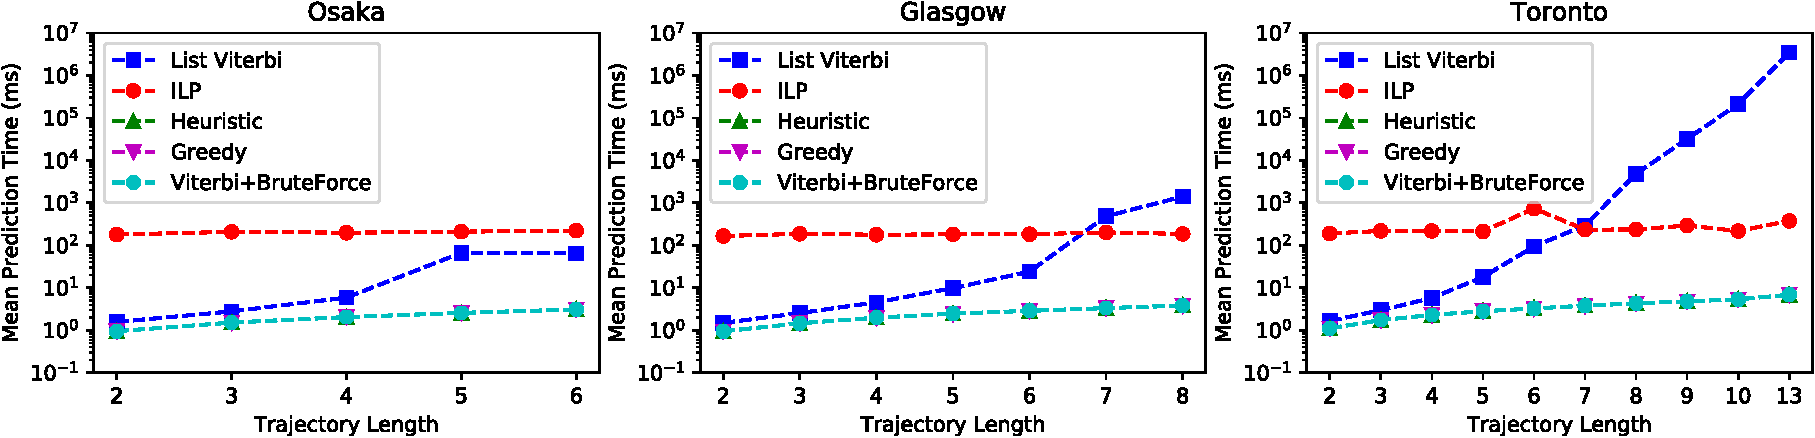
\includegraphics[width=\textwidth]{top1_inftime.pdf}
	    \captionof{figure}{Prediction time for three inference algorithms (in milliseconds)}
	    \label{fig:inftime}
	    %\captionmoveup\eqmoveup
%\end{figure*}%
%\begin{figure*}[!t]
		\quad
		\centering
		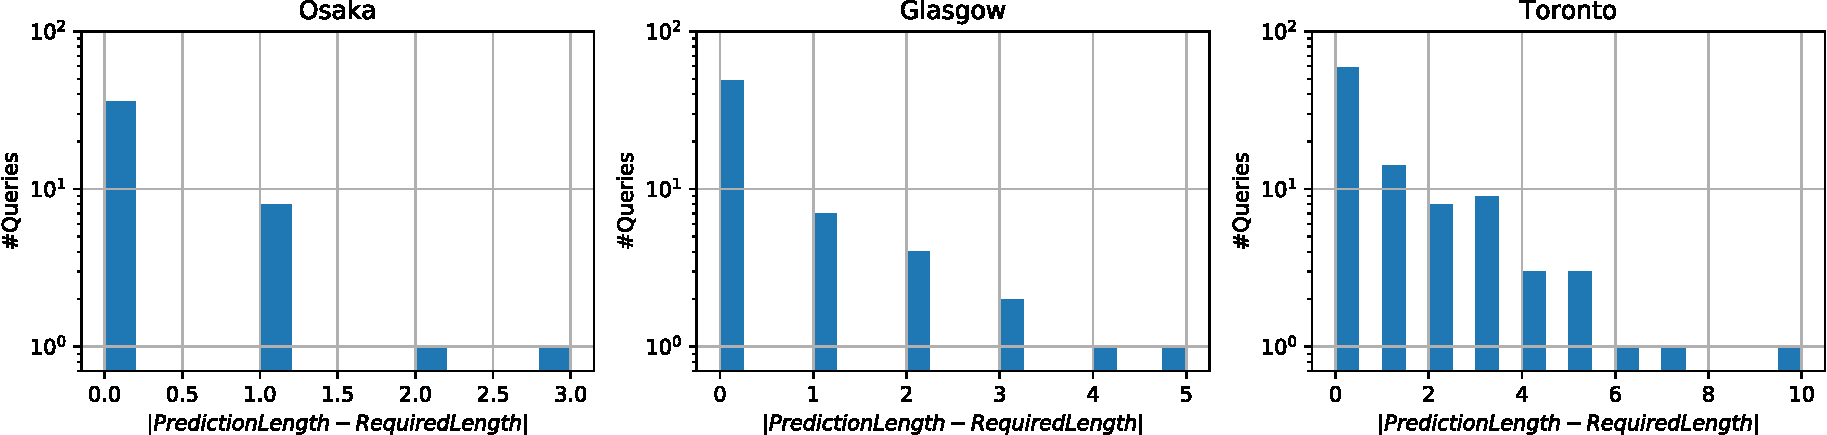
\includegraphics[width=\textwidth]{heu_lengthdiff.pdf}
	    \captionof{figure}{The difference between recommendation and required sequence length.}
	    \label{fig:length-christo}
	    %\captionmoveup\eqmoveup
%\end{figure*}%
%\begin{figure*}[!t]
		\quad
		\centering
		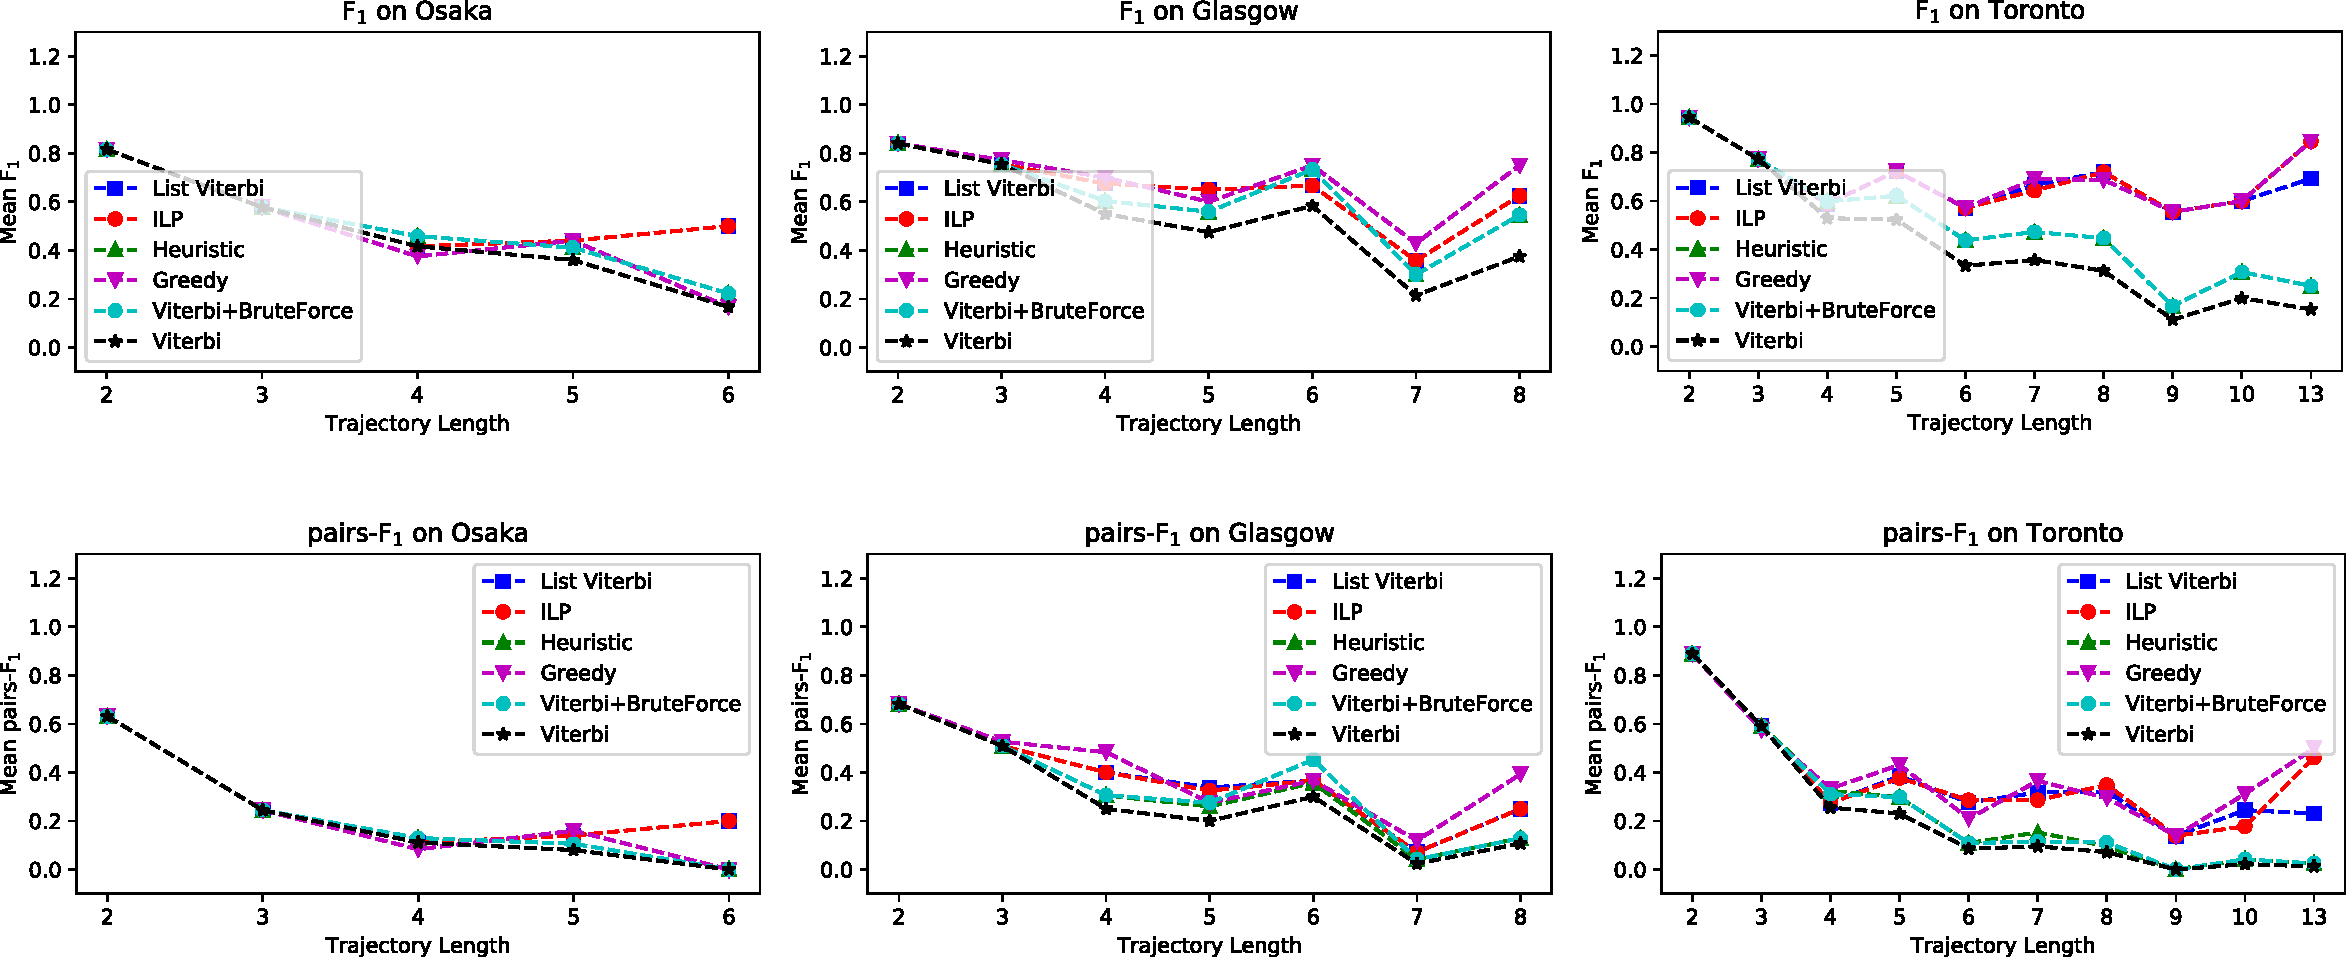
\includegraphics[width=\textwidth]{metrics.pdf}
		% 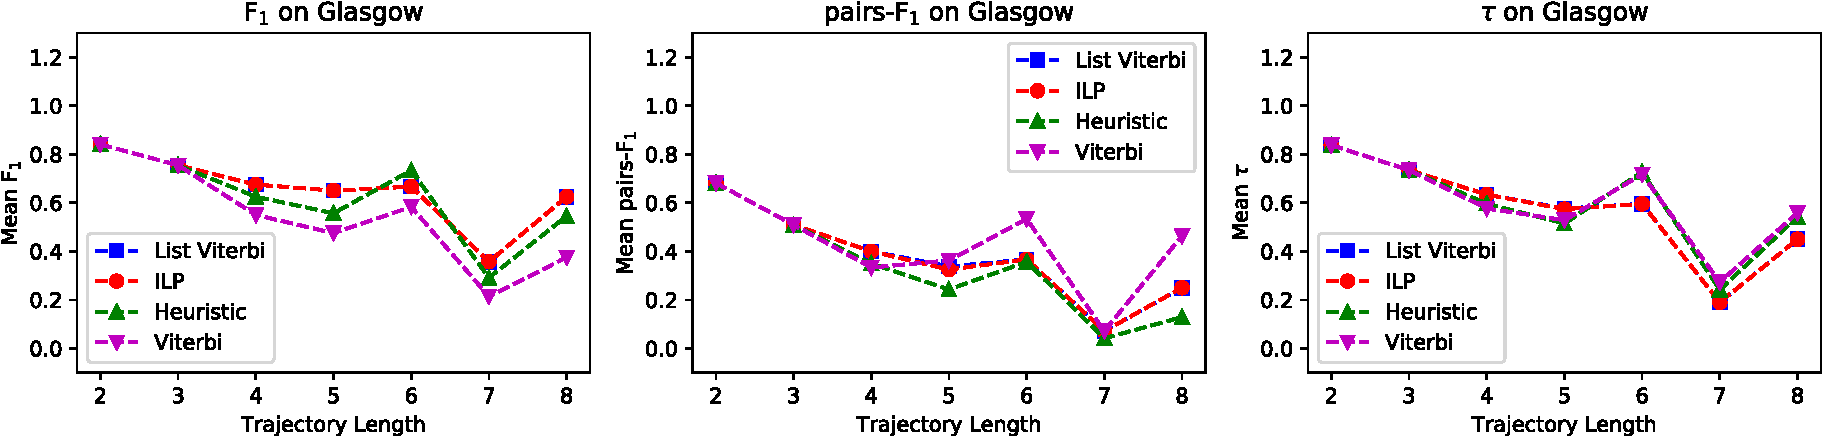
\includegraphics[width=\textwidth]{metric_d2.pdf}
		% 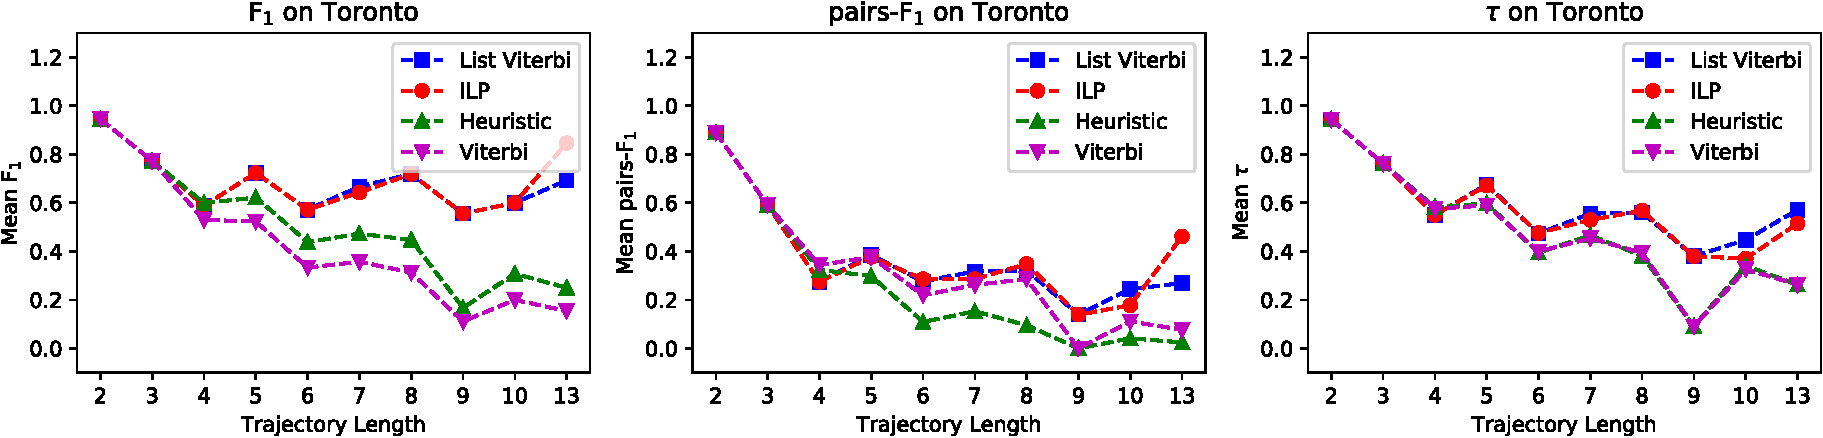
\includegraphics[width=\textwidth]{metric_d3.pdf}
	    \captionof{figure}{Accuracy versus trajectory length.}
	    \label{fig:acc-vs-length}
	    %\captionmoveup\eqmoveup
%\end{figure*}
\end{minipage}
\end{figure*}


\section{Related work}
\label{sec:related}
% related work
% describe each task with related work: the same, the different
% describe that we don't use the order of songs, conflicting findings in literature
% mainly two pieces of work:
% - music recommendation
% - playlist generation
%{\it Some related work.}


{\bf Problem type}.
\begin{itemize}
\item playlist generation given seed (\eg a seed song, artist etc.)
\item next song recommendation, given an incomplete playlist with numerous tracks, recommend the next track that the user likely to listen.
\item another closely related task is playlist continuation, given an incomplete playlist with a few tracks, recommend a list of tracks for continuing that playlist.
\end{itemize}


{\bf Method}.
\begin{itemize}
\item Markov chain based approaches + stochastic process based (\ie autodj)
\item closely related to MC approach is finding a path in a graph (\ie kdd'12) or hypergraph (\ie aotm2011)
\item ranking based, especially popularity has been proved to be very informative, further, 
artist info has been combined with popularity in (msd paper) and (cagh paper) proposed to weighting popularity by the collocation of artists, 
achieving even better performance.
\end{itemize}


{\bf Information used}.
\begin{itemize}
\item content data such as acoustic features extracted from the audio waves of songs, lyrics, genre to be shown very informative
\item artist info
\item metadata from the interaction between users and songs, such as popularity, usage stats (groove paper), generally learn latent feature 
by collaborative filtering or family of matrix factorisation techniques.
\item order of tracks in playlist, no consensus in research community, some (a few papers) report the order info is crucial to achieve high quality recommendation,
others (another bunch of papers) found the effects of track order in playlist were negligible.
Mention that we treat playlist as a set of songs in this work, and defer the investigation of track order in playlist as future work.
\end{itemize}


{\bf Problems investigated in this paper}.
\begin{itemize}
\item given a known user (a user whom we have observed a few playlists), recommend a set of songs
\item given a new user (the recsys does not have any information about the user), recommend a set of songs
\item given a set of newly released songs, recommend songs to augment current playlists.
\end{itemize}

{\bf Methods proposed}.
Two ostensibly different but in fact closely related methods,
each one can address all three tasks.
\begin{itemize}
\item classification by focusing at positive examples
\item ranking by focusing at the top
\end{itemize}




\paragraph{Gaussian process}
The AutoDJ system~\cite{platt2002learning} automatically generate playlists given one or more seed songs, 
it learns user preference from song metadata using Gaussian Process Regression,
and generates playlist with songs similar to the seed.


\paragraph{Markov chain approaches}
Playlists are modelled as random walks in a graph where vertices are songs 
and edges represents affinities between a song pairs~\cite{mcfee2011natural}.
This model can be generalised such that edges present groups of songs (by genre, user preference etc.),
which forms a hyper-graph, and a playlist is a random walk in the hyper-graph~\cite{mcfee2012hypergraph}.

The latent Markov embedding algorithm~\cite{chen2012playlist}
learns representations of songs in a latent space in which playlists are modelled as Markov chains,
playlists are then generated by sampling a paths in the latent space from locations specified by user.

\paragraph{Popularity based ranking}
Due to the \emph{long tail} distribution of songs in playlists~\cite{aoscar2010music},
similar to many applications for recommender system, 
a popularity based approach can in fact be comparably competitive~\cite{cremonesi2010performance}.
Popularity has been combined with artist information to provide strong baselines 
for playlist generation~\cite{mcfee2012million,bonnin2013evaluating,bonnin2015automated}.

\paragraph{Review}
A nice survey and review of various approaches for playlist generation~\cite{bonnin2015automated}.


\paragraph{Next song recommendation}
Next song recommendation~\cite{jannach2015beyond} approach that first scoring each song by a number of features
(\eg acoustic features, user preference of artists, social tags, song co-occurrence in playlists etc.),
then fine-tune the ranks of top-scoring songs which hopefully make the recommended next song be a coherent continuation of user's listening history.

Groove radio~\cite{ben2017groove} uses a classification approach to sequentially recommend 
the next song by predicting the probability of each possible song for a specific user, given an artist as seed.
It makes use of various information such as song metadata, usage statistics, acoustic features, popularity of song and artist,
to build features by taking into consideration of user's listening history and the playlist seed (\ie specified artist and user).
Further, this approach can deal with a cold user or artist by falling back higher levels thanks to its hierarchical architecture.


In this paper, we describe two variants of the playlist recommendation problem,
one is augmenting a playlist by recommending a subset of songs from a collection of music $\SCal$,
given the first $K$ seed songs, where $K$ can be any positive integer from 1 to the total number of songs in playlist minus 1.
% in contrast to settings where all songs except the last one are observed\cite{}, or giving a fixed number of seed songs\cite{}.
Another variant is restricting that all songs to recommend are not observed during learning,
\ie in the setting of recommending newly released songs to augment a given playlist, which is an instance of the cold-start problem.
We call the first variant \emph{playlist augmentation} and the second \emph{new song recommendation}.

% !TEX root=main.tex

{\color{red!75}
\begin{itemize}
	\item Learning
	\item diversity, MMR
	\item See whether any of the workshop topics might have problems that this paper applies.
\end{itemize}
}


% Acknowledgements should only appear in the accepted version.
%\section*{Acknowledgements}
%
%\textbf{Do not} include acknowledgements in the initial version of
%the paper submitted for blind review.
\clearpage
\bibliographystyle{ieeetr}
\bibliography{ref,ref_aditya}

\clearpage
\onecolumn

\appendix
%\section{Supplementary material to Structured Recommendation}
%\label{sec:supplement}
{\Large\bf Supplementary material to Structured Recommendation}

\setlength{\belowdisplayskip}{2pt} \setlength{\belowdisplayshortskip}{1pt}
\setlength{\abovedisplayskip}{2pt} \setlength{\abovedisplayshortskip}{1pt}

\section{Model learning and prediction}
\label{sec:supplement}

In this section, we describe the 1-slack formulation for the proposed SR model 
and the details of the list Viterbi algorithm.

\subsection{1-slack formulation for the SR model}
\label{ssec:1slack_sr}

We can use \emph{one} slack variable to represent the sum of the $N$ hinge losses:
\begin{equation*}
%%\label{eq:hingeloss}
%%\resizebox{1.1\linewidth}{!}{
%%\begin{minipage}{\linewidth}
%\begin{align*}
\xi_i = \max \left( 0, \, 
        \max_{\bar{\y} \in \mathcal{Y}}
        \left\{ \Delta(\y^{(i)}, \bar{\y}) + \w^\top \Psi(\x^{(i)}, \bar{\y}) \right\} - \w^\top \Psi(\x^{(i)}, \y^{(i)}) \right).
%\end{align*}
%%\end{minipage}
%%}
\end{equation*}
Which results in the 1-slack formulation for the SR model:
\begin{equation*}
%%\label{eq:1slack_ml}
\resizebox{0.9\linewidth}{!}{$
\begin{aligned}
\min_{\w, \, \xi \ge 0} ~\frac{1}{2} \w^\top \w + C \xi, ~~s.t.~ \frac{1}{N} \left( \sum_{i,j} \w^\top \Psi(\x^{(i)}, \y^{(ij)}) - \w^\top \Psi(\x^{(i)}, \bar{\y}^{(i)}) \right) 
  \ge \frac{1}{N} \sum_{i,j} \Delta(\y^{(ij)}, \bar{\y}^{(i)}) - \xi.
\end{aligned}
$}
\end{equation*}


\subsection{The list Viterbi algorithm}
\label{sec:listviterbi-supp}

We make use of the list Viterbi in four situations:
\begin{enumerate}
  \item To avoid sequence with loops during the prediction phase of the SP and SR models
  \item To make top-$k$ prediction using the SP and SR models
  \item To eliminate known ground truths during the training phase (\ie loss augmented inference) of the SR and \textsc{SRpath} models
  \item To avoid sequence with loops during the training phase (\ie loss augmented inference) of the \textsc{SPpath} and \textsc{SRpath} models
\end{enumerate}

%%There are two general approaches for generalising Viterbi decoding to when we require $k$
%%sequences to be decoded: by maintaining $k$ paths through the trellis while decoding; or by
%%careful book keeping of the best $k-1$ paths through the trellis found so far and avoiding them.
%%We choose the latter approach as it is more memory efficient.

The serial list Viterbi algorithm~\cite{nilsson2001sequentially,seshadri1994list} maintains
a heap (\ie priority queue) of potential solutions, which are then checked for the desired property (for example
whether there are loops). Once the requisite number of trajectories with the desired
property are found, the algorithm terminates (for example once $k$ trajectories without loops are found when performing top-k prediction)
The heap is initialised by running forward-backward (Algorithm~\ref{alg:forward-backward}) followed by the vanilla Viterbi (Algorithm~\ref{alg:viterbi}).

\begin{algorithm}[htbp]
\caption{Forward-backward procedure~\cite{rabiner1989tutorial}}
\label{alg:forward-backward}
\begin{algorithmic}[1]
  \STATE $\forall p_j \in \mathcal{P},~ \alpha_t(p_j) =
          \begin{cases}
          0,~ t = 1 \\
          \max_{p_i \in \mathcal{P}} \left\{ \alpha_{t-1}(p_i) + \mathbf{w}_{ij}^\top \psi_{ij}(\mathbf{x}, p_i, p_j) +
          \mathbf{w}_j^\top \psi_j(\mathbf{x}, p_j) \right\},~ t=2,\dots,l
          \end{cases}$

  \STATE $\forall p_i \in \mathcal{P},~ \beta_t(p_i) =
          \begin{cases}
          0,~ t = l \\
          \max_{p_j \in \mathcal{P}} \left\{ \mathbf{w}_{ij}^\top \psi_{ij}(\mathbf{x}, p_i, p_j) +
          \mathbf{w}_j^\top \psi_j(\mathbf{x}, p_j) + \beta_{t+1}(p_j) \right\},~ t = l-1,\dots,1
          \end{cases}$

  %\STATE $\forall p_i \in \mathcal{P},~ f_t(p_i) = \alpha_t(p_i) + \beta_t(p_i),~ t = 1,\dots,K$
  \STATE $\forall p_i, p_j \in \mathcal{P},~ f_{t,t+1}(p_i, p_j) = \alpha_t(p_i) + \mathbf{w}_{ij}^\top \psi_{ij}(\mathbf{x}, p_i, p_j) +
                                \mathbf{w}_j^\top \psi_j(\mathbf{x}, p_j) + \beta_{t+1}(p_j),~ t = 1,\dots,l-1$
\end{algorithmic}
\end{algorithm}

\begin{algorithm}[htbp]
\caption{Viterbi}
\label{alg:viterbi}
\begin{algorithmic}[1]
  \STATE $y_t^1 = \begin{cases}
                  s,~ t = 1 \\
  %                \argmax_{p \in \mathcal{P}} \left\{ f_{1,2}(s, p) \right\},~ t = 2, \\
                  \argmax_{p \in \mathcal{P}} \left\{ f_{t-1,t}(y_{t-1}^1, p) \right\},~ t = 2,\dots,l
                  \end{cases}$

  %\STATE $r^1 = \max_{p \in \mathcal{P}} \left\{ f_K(p) \right\}~~~ \triangleright$ $r^1$ is the score/priority of $\mathbf{y}^1$
  \STATE $r^1 = \max_{p \in \mathcal{P}} \left\{ \alpha_{l}(p) \right\}~~~ \triangleright$ $r^1$ is the score/priority of $\mathbf{y}^1$
\end{algorithmic}
\end{algorithm}

Given an existing heap containing potential trajectories,
list Viterbi maintains a set of POIs $S$ to exclude, which is updated
sequentially by considering the front sequence of the heap.

Recall that for trajectory recommendation we are given the query $\mathbf{x}=(s, l)$, where
$s$ is the starting POI from the set of POIs $\mathcal{P}$,
and $l$ is the desired length of the trajectory.
We assume the score function is of the form $\mathbf{w}^\top \Psi$ where $\Psi$ is the joint
feature vector. $\mathbf{w}$ could be the value of the weight in the current iteration in training,
or the learned weight vector during prediction.

The list Viterbi algorithm for performing top-$k$ prediction is described in Algorithm~\ref{alg:listviterbi}.
To eliminating known ground truths in loss augmented inference,
we modify the forward-backward procedure (Algorithm~\ref{alg:forward-backward}) to account for the loss term $\Delta(\cdot,\cdot)$,
and Algorithm~\ref{alg:viterbi} and Algorithm~\ref{alg:listviterbi} can be used without modification.

\begin{algorithm}[htbp]
\caption{The list Viterbi algorithm for top-$K$ prediction~\cite{nilsson2001sequentially,seshadri1994list}}
\label{alg:listviterbi}
\begin{algorithmic}[1]
\STATE \textbf{Input}: $\mathbf{x}=(s, l),~ \mathcal{P},~ \mathbf{w},~ \Psi, ~K$
%\STATE Initialise score matrices $\alpha,~ \beta,~ f_t,~ f_{t, t+1}$, a max-heap $H,~ k=0$.
\STATE Initialise score matrices $\alpha,~ \beta,~ f_{t, t+1}$, a max-heap $H$, result set $R$, $k=0$.
\STATE $\triangleright$ Do the forward-backward procedure (Algorithm~\ref{alg:forward-backward})
\STATE $\triangleright$ Identify the best (scored) trajectory $\mathbf{y}^1=(y_1^1,\dots,y_l^1)$
  with Viterbi (Algorithm~\ref{alg:viterbi}). This may be a trajectory that violates the desired condition.
\STATE $H.\textit{push}\left(r^1,~ (\mathbf{y}^1, \textsc{nil}, \emptyset) \right)$
\STATE Set $R=\emptyset$, the list of trajectories to be returned.
\WHILE{$H \ne \emptyset$ \textbf{and} $k < \,|\mathcal{P}|^{l-1} - \prod_{t=2}^l (|\mathcal{P}|-t+1) + K$}
    \STATE $r^k,~ (\mathbf{y}^k, I, S) = H.\textit{pop}()~~~ \triangleright$
           $r^k$ is the score of $\mathbf{y}^k=(y_1^k,\dots,y_l^k)$, $I$ is the partition index, and $S$ is the exclude set
    \STATE $k = k + 1$
    \STATE Add $\mathbf{y}^k$ to $R$ if it satisfies the desired property
    \RETURN $R$ if it contains the required number of trajectories
    \STATE $I' = \begin{cases}
                  2, & I = \textsc{nil} \\
                  I, & \text{otherwise}
                 \end{cases}$

    \FOR{$t = I',\dots,l$}
        \STATE $S' = \begin{cases}
                      S \cup \{ y_t^k \}, & t = I' \\
                      \{ y_t^k \},        & \text{otherwise}
                     \end{cases}$

        \STATE $y'_j = \begin{cases}
                            y_j^k,                                                                             & j=1,\dots,t-1 \\
                            \argmax_{p \in \mathcal{P} \setminus S'} \left\{ f_{t-1,t}(y_{t-1}^k, p) \right\}, & j=t \\
                            \argmax_{p \in \mathcal{P}} \left\{ f_{j-1, j}(y'_{j-1}, p) \right\},              & j=t+1,\dots,l
                \end{cases}$
        %\STATE $\bar{r} = \begin{cases}
        %                  f_{t-1,t}(y_{t-1}^k, \bar{y}_t),&I = \textsc{nil} \\
        %                  r^k + f_{t-1,t}(y_{t-1}^k, \bar{y}_t) - f_{t-1,t}(y_{t-1}^k, y_t^k), &\text{otherwise}
        %                  \end{cases}$
        \STATE \vspace{3pt}$r' = r^k + f_{t-1,t}(y_{t-1}^k, y'_t) - f_{t-1,t}(y_{t-1}^k, y_t^k)$

        \STATE \vspace{3pt}$H.\textit{push}(r', (\y', t, S') )$ \vspace{2pt}
    \ENDFOR
\ENDWHILE
\end{algorithmic}
\end{algorithm}

\clearpage

\section{Experiment}

In this section, we describe trajectory dataset used in experiments as well as features for each methods.
In addition, the details of evaluation and empirical results are also described.

\subsection{Photo trajectory dataset and features}
\label{sec:feature}

\textbf{Dataset}.
In the interests of reproducibility we present further details of our empirical experiment.
The histogram of the number of trajectories per query is shown in Figure~\ref{fig:hist_query},
where we can see each query has 4-9 ground truths (\ie trajectories) on average, and 30-60 trajectories at most.
The histogram of trajectory length (\ie the number of POIs in a trajectory) is shown in Figure~\ref{fig:hist_length},
where we can see the majority are short trajectories (\ie length $\le$ 5).

% histogram of #ground truth
\begin{figure}[t]
	\centering
	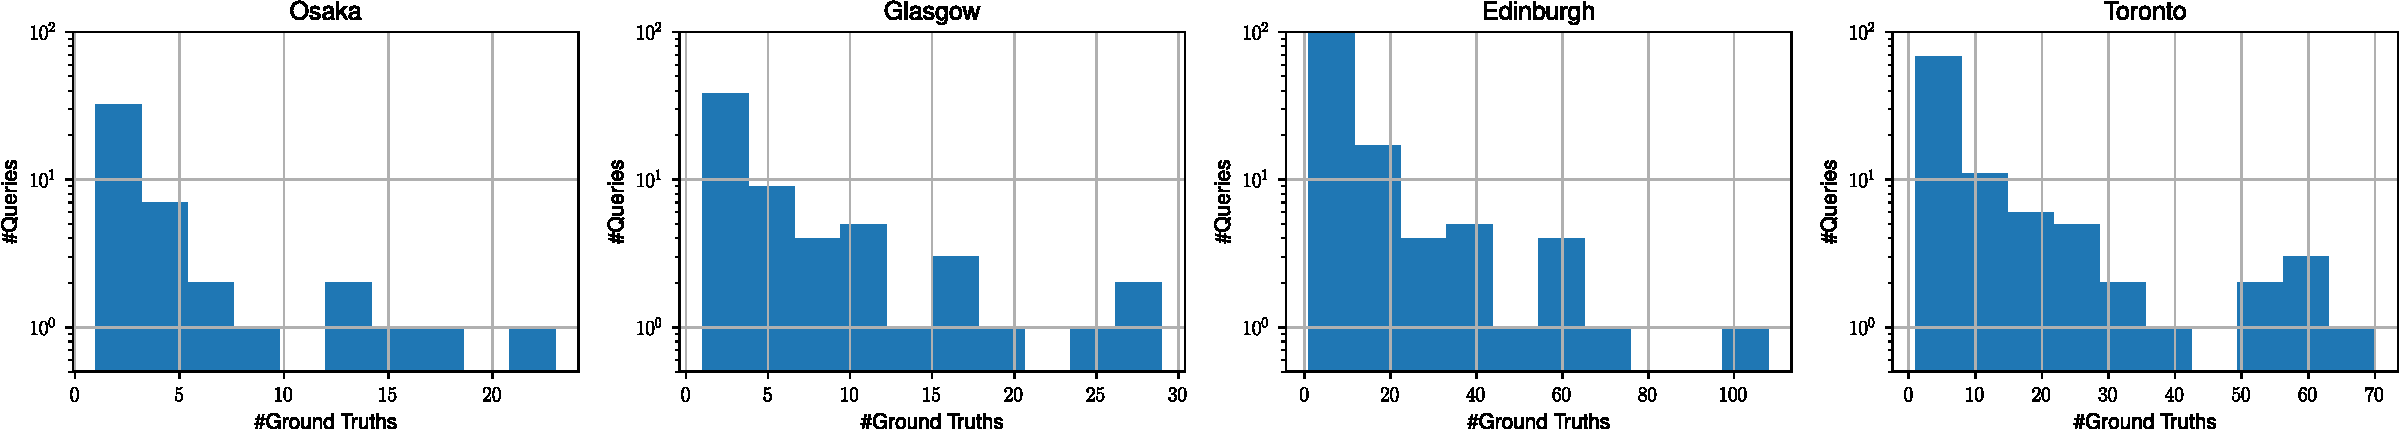
\includegraphics[width=.7\linewidth]{hist_query.pdf}
	\caption{Histograms of the number of trajectories per query.}
	\label{fig:hist_query}
\end{figure}


% histogram of trajectory length
\begin{figure}[t]
	\centering
	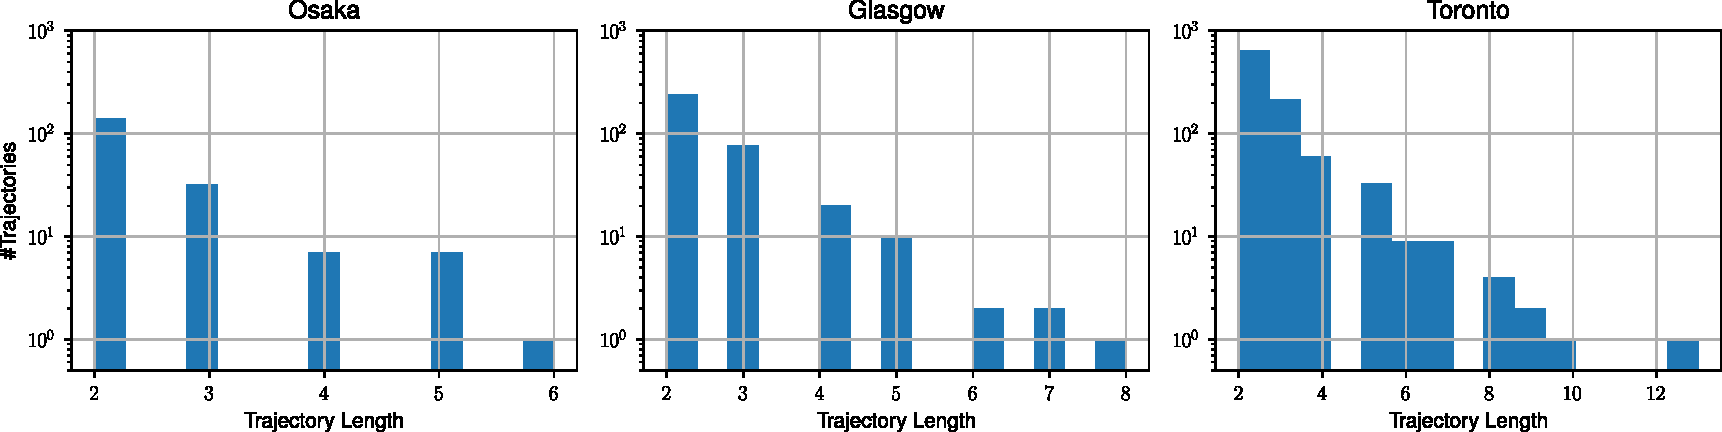
\includegraphics[width=.7\linewidth]{hist_length.pdf}
	\caption{Histograms of trajectory length.}
	\label{fig:hist_length}
\end{figure}


\textbf{Features}.
The POI-query features used by \textsc{PoiRank}, SP and SR methods and their extensions 
(\ie the \textsc{SPpath} and \textsc{SRpath} models) are shown in Table~\ref{tab:poifeature},
pairwise features used in SP and SR methods and their extensions are shown in Table~\ref{tab:tranfeature}.

\begin{table*}[!h]
\caption{POI-query features: features of POI $p$ with respect to query $(s,l)$}
\label{tab:poifeature}
\centering
\small
\setlength{\tabcolsep}{10pt} % tweak the space between columns
\begin{tabular}{l|l} \hline
\textbf{Feature}       & \textbf{Description} \\ \hline
\texttt{category}      & one-hot encoding of the category of $p$ \\
\texttt{neighbourhood} & one-hot encoding of the POI cluster that $p$ resides in \\
\texttt{popularity}    & logarithm of POI popularity of $p$ \\
\texttt{nVisit}        & logarithm of the total number of visit by all users at $p$ \\
\texttt{avgDuration}  & logarithm of the average visit duration at $p$ \\
\hline
%\texttt{nOccurrence}            & the number of times $p$ occurred in a trajectory that satisfies the query \\ DON'T know given new query

\texttt{trajLen}           & trajectory length $l$, i.e., the number of POIs required \\
\texttt{sameCatStart}      & $1$ if the category of $p$ is the same as that of $s$, $-1$ otherwise \\
\texttt{sameNeighbourhoodStart} & $1$ if $p$ resides in the same POI cluster as $s$, $-1$ otherwise \\
\texttt{diffPopStart}    & real-valued difference in POI popularity of $p$ from that of $s$ \\
\texttt{diffNVisitStart}        & real-valued difference in the total number of visit at $p$ from that at $s$ \\
\texttt{diffDurationStart}  & real-valued difference in average duration at $p$ from that at $s$ \\
\texttt{distStart}          & distance between $p$ and $s$, calculated using the Haversine formula \\
\hline
\end{tabular}
\end{table*}



\begin{table}[!h]
\caption{Pairwise POI features}
\label{tab:tranfeature}
\centering
\small
\setlength{\tabcolsep}{2pt} % tweak the space between columns
\begin{tabular}{l|l} \hline
\textbf{Feature}       & \textbf{Description} \\ \hline
\texttt{category}      & category of POI \\
\texttt{neighbourhood} & the cluster that a POI resides in \\
\texttt{popularity}    & (discretised) popularity of POI \\
\texttt{nVisit}        & (discretised) total number of visit at POI \\
\texttt{avgDuration}  & (discretised) average duration at POI \\ \hline
\end{tabular}
\end{table}


\clearpage
\subsection{Evaluation settings}
\label{sec:metric}

\textbf{Top-k prediction for baselines}.
\begin{itemize}
\item To perform top-$k$ prediction with \textsc{Random} baseline, we simply repeat the \textsc{Random} method $k$ times.
\item To perform top-$k$ prediction with \textsc{Popularity} and \textsc{PoiRank}, we make use of the list Viterbi algorithm 
      (Algorithm~\ref{alg:listviterbi} to get $k$ best scored paths, in particular, 
      for \textsc{Popularity}, the score of a path is the accumulated popularity of all POIs in the path; 
      for \textsc{PoiRank}, the score of a path is the likelihood 
      (the ranking scores for POIs are first transformed into a probability distribution using the softmax function, as described in~\cite{cikm16paper}).
\end{itemize}

To evaluate the performance of a certain recommendation algorithm,
we need to measure the similarity (or loss) given prediction $\hat{\mathbf{y}}$
and ground truth $\mathbf{y}$.


\textbf{F$_1$ score on points}.
F$_1$ score on points~\cite{ijcai15} cares about only the set of correctly recommended POIs.
%%Let $\texttt{set}(\mathbf{y})$ denote the set of POIs in trajectory $\mathbf{y}$, F$_1$ score on points is defined as
\begin{equation*}
F_1(\mathbf{y}, \hat{\mathbf{y}}) = \frac{2  P_{\textsc{point}}  R_{\textsc{point}}}{P_{\textsc{point}} + R_{\textsc{point}}}
%~~\text{where}~
%P_{\textsc{point}} = \frac{| \texttt{set}(\hat{\mathbf{y}}) \cap \texttt{set}(\mathbf{y}) |}{| \texttt{set}(\hat{\mathbf{y}}) |}~\text{and}~
%R_{\textsc{point}} = \frac{| \texttt{set}(\hat{\mathbf{y}}) \cap \texttt{set}(\mathbf{y}) |}{| \texttt{set}(\mathbf{y}) |}.
\end{equation*}
where $P_\textsc{point}$, $R_\textsc{point}$ are respectively the precision and recall for points in $\hat\y$ and $\y$.
If $| \hat{\mathbf{y}} | = | \mathbf{y} |$, this metric is just the unordered Hamming loss,
i.e., Hamming loss between two binary indicator vectors of size $| \mathcal{P} |$.

\textbf{F$_1$ score on pairs}.
To take into account the orders in recommended sequence, 
we also use the F$_1$ score on pairs~\cite{cikm16paper} measure, which considers the set of correctly predicted POI pairs,
\begin{equation*}
\text{pairs-F}_1(\mathbf{y}, \hat{\mathbf{y}}) = \frac{2 P_{\textsc{pair}} R_{\textsc{pair}}}{P_{\textsc{pair}} + R_{\textsc{pair}}}
%~~\text{where}~
%P_{\textsc{pair}} = \frac{N_c} {| \texttt{set}(\hat{\mathbf{y}}) | (| \texttt{set}(\hat{\mathbf{y}}) | - 1) / 2}~\text{and}~
%R_{\textsc{pair}} = \frac{N_c} {| \texttt{set}(\mathbf{y}) | (| \texttt{set}(\mathbf{y}) | - 1) / 2},
\end{equation*}
where $P_\textsc{point}$, $R_\textsc{point}$ are respectively the precision and recall for all possible pairs of $\hat\y$ and $\y$.
%%\eat{
%%and $N_c = \sum_{j=1}^{| \mathbf{y} | - 1} \sum_{k=j+1}^{| \mathbf{y} |} \llb y_j \prec_{\bar{\mathbf{y}}} y_k \rrb$,
%%here $y_j \prec_{\bar{\mathbf{y}}} y_k$ denotes that POI $y_j$ appears before POI $y_k$ in trajectory $\bar{\mathbf{y}}$.
%%We define pairs-F$_1 = 0$ when $N_c = 0$.
%%}


\textbf{Kendall's $\tau$ with ties}
Alternatively, we can cast a trajectory $\y = y_{1:l}$ as a ranking of POIs in $\mathcal{P}$,
where $y_j$ has a rank $| \mathcal{P} | - j + 1$ and any other POI $p \notin \mathbf{y}$ has a rank $0$ ($0$ is an arbitrary choice),
then we can make use of ranking evaluation metrics such as Kendall's $\tau$ by taking care of ties in ranks.
In particular, given a prediction $\hat\y = \hat{y_{1:l}}$ and ground truth $\y = y_{1:l}$,
we produce two ranks for $\mathbf{y}$ and $\hat{\mathbf{y}}$ with respect to 
a specific ordering of POIs $(p_1, p_2, \dots, p_{|\mathcal{P}|})$:
\begin{align*}
r_i       &= \sum_{j=1}^l (| \mathcal{P} | - j + 1)  \llb p_i = y_j \rrb,~
i = 1, \dots, | \mathcal{P} | \\
\hat{r}_i &= \sum_{j=1}^l (| \mathcal{P} | - j + 1)  \llb p_i = \hat{y}_j \rrb,~
i = 1, \dots, | \mathcal{P} |
\end{align*}
where POIs not in $\mathbf{y}$ will have a rank of $0$.
Then we compute the following metrics:
\begin{itemize}
\item the number of concordant pairs \(
      C = \frac{1}{2} \sum_{i,j} \left(\llb r_i < r_j \rrb  \llb \hat{r}_i < \hat{r}_j \rrb +
                      \llb r_i > r_j \rrb  \llb \hat{r}_i > \hat{r}_j \rrb \right) \)
\item the number of discordant pairs \(
      D = \frac{1}{2} \sum_{i,j} \left(\llb r_i < r_j \rrb  \llb \hat{r}_i > \hat{r}_j \rrb +
                      \llb r_i > r_j \rrb  \llb \hat{r}_i < \hat{r}_j \rrb \right) \)
\item the number of ties in ground truth $\y$: \(
      T_{\mathbf{y}} = \frac{1}{2} \sum_{i \ne j} \llb r_i = r_j \rrb 
%                     = \frac{1}{2} \sum_{i \ne j} \llb r_i = 0 \rrb  \llb r_j = 0 \rrb 
                     = \frac{1}{2} \left( |\mathcal{P}| - l \right) \left( |\mathcal{P}| - l - 1 \right) \)
\item the number of ties in prediction $\hat\y$: \(
      T_{\hat{\mathbf{y}}} = \frac{1}{2} \sum_{i \ne j} \llb \hat{r}_i = \hat{r}_j \rrb 
%                           = \frac{1}{2} \sum_{i \ne j} \llb \hat{r}_i = 0 \rrb  \llb \hat{r}_j = 0 \rrb 
                           = \frac{1}{2} \left( |\mathcal{P}| - l \right) \left( |\mathcal{P}| - l - 1 \right) \)
\item the number of ties in both $\y$ and $\hat\y$: \(
      T_{\mathbf{y},\hat{\mathbf{y}}} = \frac{1}{2} \sum_{i \ne j} \llb r_i = r_j \rrb  \llb \hat{r}_i = \hat{r}_j \rrb \)
%                                      = \frac{1}{2} \sum_{i \ne j} \llb r_i = 0 \rrb  \llb r_j = 0 \rrb
%                                        \llb \hat{r}_i = 0 \rrb  \llb \hat{r}_j = 0 \rrb \)
\end{itemize}
Kendall's $\tau$ (version $b$)~\cite{kendall1945,agresti2010analysis} is
\begin{equation*}
\tau_b(\mathbf{y}, \hat{\mathbf{y}}) = \frac{C - D}{\sqrt{(C + D + T) (C + D + U)}},
\end{equation*}
where $T = T_{\mathbf{y}} - T_{\mathbf{y},\hat{\mathbf{y}}}$ and $U = T_{\hat{\mathbf{y}}} - T_{\mathbf{y},\hat{\mathbf{y}}}$.

%Furthermore, F$_1$ score on points can be written as
%\begin{equation*}
%F_1(\mathbf{y}, \hat{\mathbf{y}}) = \frac{1}{l} \sum_i \llb r_i > 0 \rrb  \llb \hat{r}_i > 0 \rrb,
%\end{equation*}
%and F$_1$ score on pairs can be written as
%\begin{align*}
%& \text{pairs-F}_1(\mathbf{y}, \hat{\mathbf{y}}) \\
%&= \left( \frac{1}{2} \sum_{i,j} \llb r_i < r_j \rrb  \llb r_i > 0 \rrb \llb \hat{r}_i < \hat{r}_j \rrb  \llb \hat{r}_i > 0 \rrb \right. \\
%&  \left. ~+ \frac{1}{2} \sum_{i,j} \llb r_i > r_j \rrb  \llb r_j > 0 \rrb \llb \hat{r}_i > \hat{r}_j \rrb  \llb \hat{r}_j > 0 \rrb \right)
%   \cdot \frac{1}{l(l-1)/2} \\
%&= \frac{\sum_{i,j} \llb r_i < r_j \rrb  \llb r_i > 0 \rrb \llb \hat{r}_i < \hat{r}_j \rrb  \llb \hat{r}_i > 0 \rrb +
%         \sum_{i,j} \llb r_i > r_j \rrb  \llb r_j > 0 \rrb \llb \hat{r}_i > \hat{r}_j \rrb  \llb \hat{r}_j > 0 \rrb}
%        {l(l-1)}
%\end{align*}

\clearpage
\subsection{Empirical results}

\textbf{The effects of $k$ for top-$k$ prediction}.
The performance of baselines and structured recommendation algorithms for top-$k$ ($k=1,3,5,10$) 
prediction are shown in the following tables.
Bold entries: \textbf{best} performing method for each metric; italicised entries: the \textit{next best}. 

% topk evaluation table
\begin{table*}[!h]
\caption{Results on trajectory recommendation datasets on best of top-1.}
\centering
\scriptsize
\setlength{\tabcolsep}{3pt} % tweak the space between columns
\begin{tabular}{l|cc|ccc|ccc} \hline
& \multicolumn{8}{c}{\bf Kendall's $\tau$} \\ \hline
 & \textsc{Random} & \textsc{Popularity} & \textsc{PoiRank} & \textsc{Markov} & \textsc{SP} & \textsc{SPpath} & \textsc{SR} & \textsc{SRpath} \\ \hline
Osaka & $0.420\pm0.030$ & $0.566\pm0.034$ & $\mathbf{0.644\pm0.040}$ & $0.600\pm0.036$ & $0.525\pm0.037$ & $0.525\pm0.039$ & $0.608\pm0.042$ & $\mathit{0.613\pm0.044}$ \\
Glasgow & $0.430\pm0.031$ & $0.644\pm0.036$ & $\mathbf{0.733\pm0.030}$ & $0.623\pm0.030$ & $0.564\pm0.029$ & $0.615\pm0.034$ & $0.708\pm0.031$ & $\mathit{0.712\pm0.031}$ \\
Toronto & $0.394\pm0.025$ & $0.626\pm0.023$ & $\mathit{0.714\pm0.024}$ & $0.629\pm0.023$ & $0.543\pm0.026$ & $0.572\pm0.026$ & $0.714\pm0.026$ & $\mathbf{0.717\pm0.026}$ \\
\hline
& \multicolumn{8}{c}{\bf F$_1$ score on points} \\ \hline
Osaka & $0.459\pm0.027$ & $0.601\pm0.031$ & $\mathbf{0.678\pm0.037}$ & $0.630\pm0.034$ & $0.555\pm0.034$ & $0.558\pm0.036$ & $0.638\pm0.039$ & $\mathit{0.645\pm0.040}$ \\
Glasgow & $0.478\pm0.027$ & $0.681\pm0.032$ & $\mathbf{0.764\pm0.027}$ & $0.654\pm0.027$ & $0.604\pm0.026$ & $0.653\pm0.031$ & $0.741\pm0.028$ & $\mathit{0.743\pm0.028}$ \\
Toronto & $0.461\pm0.020$ & $0.671\pm0.021$ & $\mathit{0.756\pm0.021}$ & $0.676\pm0.021$ & $0.594\pm0.023$ & $0.623\pm0.023$ & $0.753\pm0.023$ & $\mathbf{0.757\pm0.022}$ \\
\hline
& \multicolumn{8}{c}{\bf F$_1$ score on pairs} \\ \hline
Osaka & $0.104\pm0.037$ & $0.281\pm0.051$ & $\mathbf{0.428\pm0.059}$ & $0.331\pm0.053$ & $0.243\pm0.052$ & $0.254\pm0.055$ & $0.375\pm0.059$ & $\mathit{0.401\pm0.060}$ \\
Glasgow & $0.154\pm0.035$ & $0.426\pm0.051$ & $\mathbf{0.545\pm0.046}$ & $0.368\pm0.045$ & $0.289\pm0.042$ & $0.389\pm0.048$ & $0.506\pm0.048$ & $\mathit{0.516\pm0.048}$ \\
Toronto & $0.143\pm0.025$ & $0.381\pm0.034$ & $0.503\pm0.036$ & $0.391\pm0.034$ & $0.299\pm0.033$ & $0.340\pm0.035$ & $\mathit{0.530\pm0.037}$ & $\mathbf{0.533\pm0.037}$ \\
\hline
\end{tabular}
\end{table*}


\begin{table*}[!h]
\caption{Results on trajectory recommendation datasets on best of top-3.}
\centering
\scriptsize
\setlength{\tabcolsep}{3pt} % tweak the space between columns
\begin{tabular}{l|cc|ccc|ccc} \hline
& \multicolumn{8}{c}{\bf Kendall's $\tau$} \\ \hline
 & \textsc{Random} & \textsc{Popularity} & \textsc{PoiRank} & \textsc{Markov} & \textsc{SP} & \textsc{SPpath} & \textsc{SR} & \textsc{SRpath} \\ \hline
Osaka & $0.556\pm0.037$ & $0.666\pm0.039$ & $\mathbf{0.726\pm0.042}$ & $\mathit{0.718\pm0.039}$ & $0.630\pm0.044$ & $0.698\pm0.040$ & $0.711\pm0.042$ & $0.697\pm0.042$ \\
Glasgow & $0.563\pm0.031$ & $0.693\pm0.036$ & $0.781\pm0.030$ & $0.684\pm0.032$ & $0.666\pm0.033$ & $0.688\pm0.032$ & $\mathit{0.803\pm0.029}$ & $\mathbf{0.808\pm0.030}$ \\
Toronto & $0.521\pm0.026$ & $0.670\pm0.025$ & $0.746\pm0.023$ & $0.712\pm0.023$ & $0.629\pm0.027$ & $0.650\pm0.027$ & $\mathbf{0.753\pm0.025}$ & $\mathit{0.749\pm0.024}$ \\
\hline
& \multicolumn{8}{c}{\bf F$_1$ score on points} \\ \hline
Osaka & $0.587\pm0.034$ & $0.691\pm0.035$ & $\mathbf{0.750\pm0.039}$ & $\mathit{0.740\pm0.037}$ & $0.656\pm0.040$ & $0.724\pm0.037$ & $0.735\pm0.038$ & $0.723\pm0.039$ \\
Glasgow & $0.598\pm0.028$ & $0.722\pm0.033$ & $0.803\pm0.027$ & $0.711\pm0.029$ & $0.698\pm0.030$ & $0.716\pm0.029$ & $\mathit{0.825\pm0.026}$ & $\mathbf{0.829\pm0.026}$ \\
Toronto & $0.577\pm0.022$ & $0.704\pm0.023$ & $0.776\pm0.021$ & $0.748\pm0.021$ & $0.674\pm0.023$ & $0.693\pm0.023$ & $\mathbf{0.784\pm0.022}$ & $\mathit{0.780\pm0.021}$ \\
\hline
& \multicolumn{8}{c}{\bf F$_1$ score on pairs} \\ \hline
Osaka & $0.288\pm0.055$ & $0.448\pm0.058$ & $\mathbf{0.578\pm0.060}$ & $0.538\pm0.060$ & $0.425\pm0.062$ & $0.511\pm0.059$ & $\mathit{0.549\pm0.060}$ & $0.520\pm0.059$ \\
Glasgow & $0.300\pm0.043$ & $0.524\pm0.053$ & $0.625\pm0.046$ & $0.465\pm0.048$ & $0.464\pm0.049$ & $0.481\pm0.048$ & $\mathit{0.666\pm0.045}$ & $\mathbf{0.678\pm0.045}$ \\
Toronto & $0.281\pm0.032$ & $0.473\pm0.036$ & $0.572\pm0.035$ & $0.517\pm0.035$ & $0.429\pm0.037$ & $0.461\pm0.037$ & $\mathbf{0.592\pm0.036}$ & $\mathit{0.583\pm0.036}$ \\
\hline
\end{tabular}
\end{table*}


\begin{table*}[!h]
\caption{Results on trajectory recommendation datasets on best of top-5.}
\centering
\scriptsize
\setlength{\tabcolsep}{3pt} % tweak the space between columns
\begin{tabular}{l|cc|ccc|ccc} \hline
& \multicolumn{8}{c}{\bf Kendall's $\tau$} \\ \hline
 & \textsc{Random} & \textsc{Popularity} & \textsc{PoiRank} & \textsc{Markov} & \textsc{SP} & \textsc{SPpath} & \textsc{SR} & \textsc{SRpath} \\ \hline
 & \textsc{Random} & \textsc{Popularity} & \textsc{PoiRank} & \textsc{SP} & \textsc{SPpath} & \textsc{SR} & \textsc{SRpath} \\ \hline
Osaka & $0.618\pm0.038$ & $0.674\pm0.038$ & $\mathit{0.750\pm0.040}$ & $\mathbf{0.769\pm0.036}$ & $0.678\pm0.045$ & $0.735\pm0.039$ & $0.741\pm0.039$ & $0.729\pm0.041$ \\
Glasgow & $0.623\pm0.029$ & $0.727\pm0.037$ & $0.801\pm0.030$ & $0.712\pm0.032$ & $0.727\pm0.033$ & $0.743\pm0.031$ & $\mathit{0.826\pm0.028}$ & $\mathbf{0.832\pm0.028}$ \\
Toronto & $0.574\pm0.025$ & $0.687\pm0.025$ & $0.754\pm0.023$ & $0.749\pm0.024$ & $0.662\pm0.027$ & $0.683\pm0.026$ & $\mathbf{0.778\pm0.023}$ & $\mathit{0.769\pm0.024}$ \\
\hline
& \multicolumn{8}{c}{\bf F$_1$ score on points} \\ \hline
Osaka & $0.646\pm0.035$ & $0.699\pm0.034$ & $\mathit{0.772\pm0.037}$ & $\mathbf{0.789\pm0.033}$ & $0.700\pm0.041$ & $0.757\pm0.036$ & $0.761\pm0.036$ & $0.751\pm0.037$ \\
Glasgow & $0.655\pm0.026$ & $0.754\pm0.033$ & $0.821\pm0.026$ & $0.736\pm0.029$ & $0.755\pm0.030$ & $0.770\pm0.027$ & $\mathit{0.847\pm0.024}$ & $\mathbf{0.850\pm0.025}$ \\
Toronto & $0.624\pm0.022$ & $0.719\pm0.023$ & $0.781\pm0.021$ & $0.783\pm0.021$ & $0.705\pm0.023$ & $0.724\pm0.022$ & $\mathbf{0.808\pm0.021}$ & $\mathit{0.798\pm0.021}$ \\
\hline
& \multicolumn{8}{c}{\bf F$_1$ score on pairs} \\ \hline
Osaka & $0.375\pm0.058$ & $0.459\pm0.057$ & $\mathit{0.607\pm0.058}$ & $\mathbf{0.621\pm0.055}$ & $0.507\pm0.064$ & $0.568\pm0.058$ & $0.584\pm0.058$ & $0.575\pm0.058$ \\
Glasgow & $0.377\pm0.044$ & $0.590\pm0.052$ & $0.670\pm0.045$ & $0.507\pm0.048$ & $0.563\pm0.048$ & $0.573\pm0.047$ & $\mathit{0.701\pm0.043}$ & $\mathbf{0.715\pm0.044}$ \\
Toronto & $0.343\pm0.034$ & $0.500\pm0.036$ & $0.590\pm0.034$ & $0.581\pm0.034$ & $0.483\pm0.037$ & $0.509\pm0.037$ & $\mathbf{0.624\pm0.035}$ & $\mathit{0.609\pm0.035}$ \\
\hline
\end{tabular}
\end{table*}


\begin{table*}[!h]
\caption{Results on trajectory recommendation datasets on best of top-10.}
\centering
\scriptsize
\setlength{\tabcolsep}{3pt} % tweak the space between columns
\begin{tabular}{l|cc|ccc|ccc} \hline
& \multicolumn{8}{c}{\bf Kendall's $\tau$} \\ \hline
 & \textsc{Random} & \textsc{Popularity} & \textsc{PoiRank} & \textsc{Markov} & \textsc{SP} & \textsc{SPpath} & \textsc{SR} & \textsc{SRpath} \\ \hline
Osaka & $0.685\pm0.035$ & $0.768\pm0.038$ & $0.787\pm0.037$ & $\mathbf{0.824\pm0.031}$ & $0.749\pm0.043$ & $0.791\pm0.036$ & $0.777\pm0.036$ & $\mathit{0.803\pm0.034}$ \\
Glasgow & $0.703\pm0.029$ & $0.748\pm0.036$ & $0.830\pm0.029$ & $0.781\pm0.031$ & $0.790\pm0.030$ & $0.787\pm0.029$ & $\mathbf{0.868\pm0.026}$ & $\mathit{0.853\pm0.026}$ \\
Toronto & $0.652\pm0.024$ & $0.719\pm0.024$ & $0.784\pm0.023$ & $0.789\pm0.022$ & $0.697\pm0.027$ & $0.719\pm0.026$ & $\mathbf{0.802\pm0.022}$ & $\mathit{0.797\pm0.022}$ \\
\hline
& \multicolumn{8}{c}{\bf F$_1$ score on points} \\ \hline
Osaka & $0.703\pm0.032$ & $0.786\pm0.034$ & $0.804\pm0.034$ & $\mathbf{0.840\pm0.029}$ & $0.770\pm0.039$ & $0.809\pm0.033$ & $0.793\pm0.033$ & $\mathit{0.820\pm0.031}$ \\
Glasgow & $0.731\pm0.026$ & $0.771\pm0.033$ & $0.847\pm0.025$ & $0.800\pm0.028$ & $0.810\pm0.027$ & $0.807\pm0.026$ & $\mathbf{0.883\pm0.023}$ & $\mathit{0.868\pm0.023}$ \\
Toronto & $0.696\pm0.021$ & $0.746\pm0.022$ & $0.807\pm0.020$ & $0.819\pm0.019$ & $0.733\pm0.023$ & $0.755\pm0.022$ & $\mathbf{0.828\pm0.019}$ & $\mathit{0.823\pm0.020}$ \\
\hline
& \multicolumn{8}{c}{\bf F$_1$ score on pairs} \\ \hline
Osaka & $0.451\pm0.057$ & $0.626\pm0.055$ & $0.661\pm0.056$ & $\mathbf{0.693\pm0.051}$ & $0.620\pm0.061$ & $0.664\pm0.055$ & $0.637\pm0.055$ & $\mathit{0.671\pm0.053}$ \\
Glasgow & $0.495\pm0.046$ & $0.623\pm0.051$ & $0.726\pm0.043$ & $0.635\pm0.048$ & $0.658\pm0.046$ & $0.648\pm0.045$ & $\mathbf{0.770\pm0.039}$ & $\mathit{0.746\pm0.041}$ \\
Toronto & $0.438\pm0.034$ & $0.546\pm0.036$ & $0.646\pm0.034$ & $0.644\pm0.033$ & $0.530\pm0.037$ & $0.552\pm0.036$ & $\mathbf{0.660\pm0.033}$ & $\mathit{0.656\pm0.034}$ \\
\hline
\end{tabular}
\end{table*}


%\clearpage
\textbf{Performance on short and long trajectories}.
The performance of baselines and structured recommendation algorithms 
for short (length $<$ 5) and long (length $\ge$ 5) trajectories 
with top-$k$ ($k=1:10$) prediction are shown in the following figures.

% topk evaluation plots
%\includepdf[pages={1-},scale=0.75]{plots.pdf}
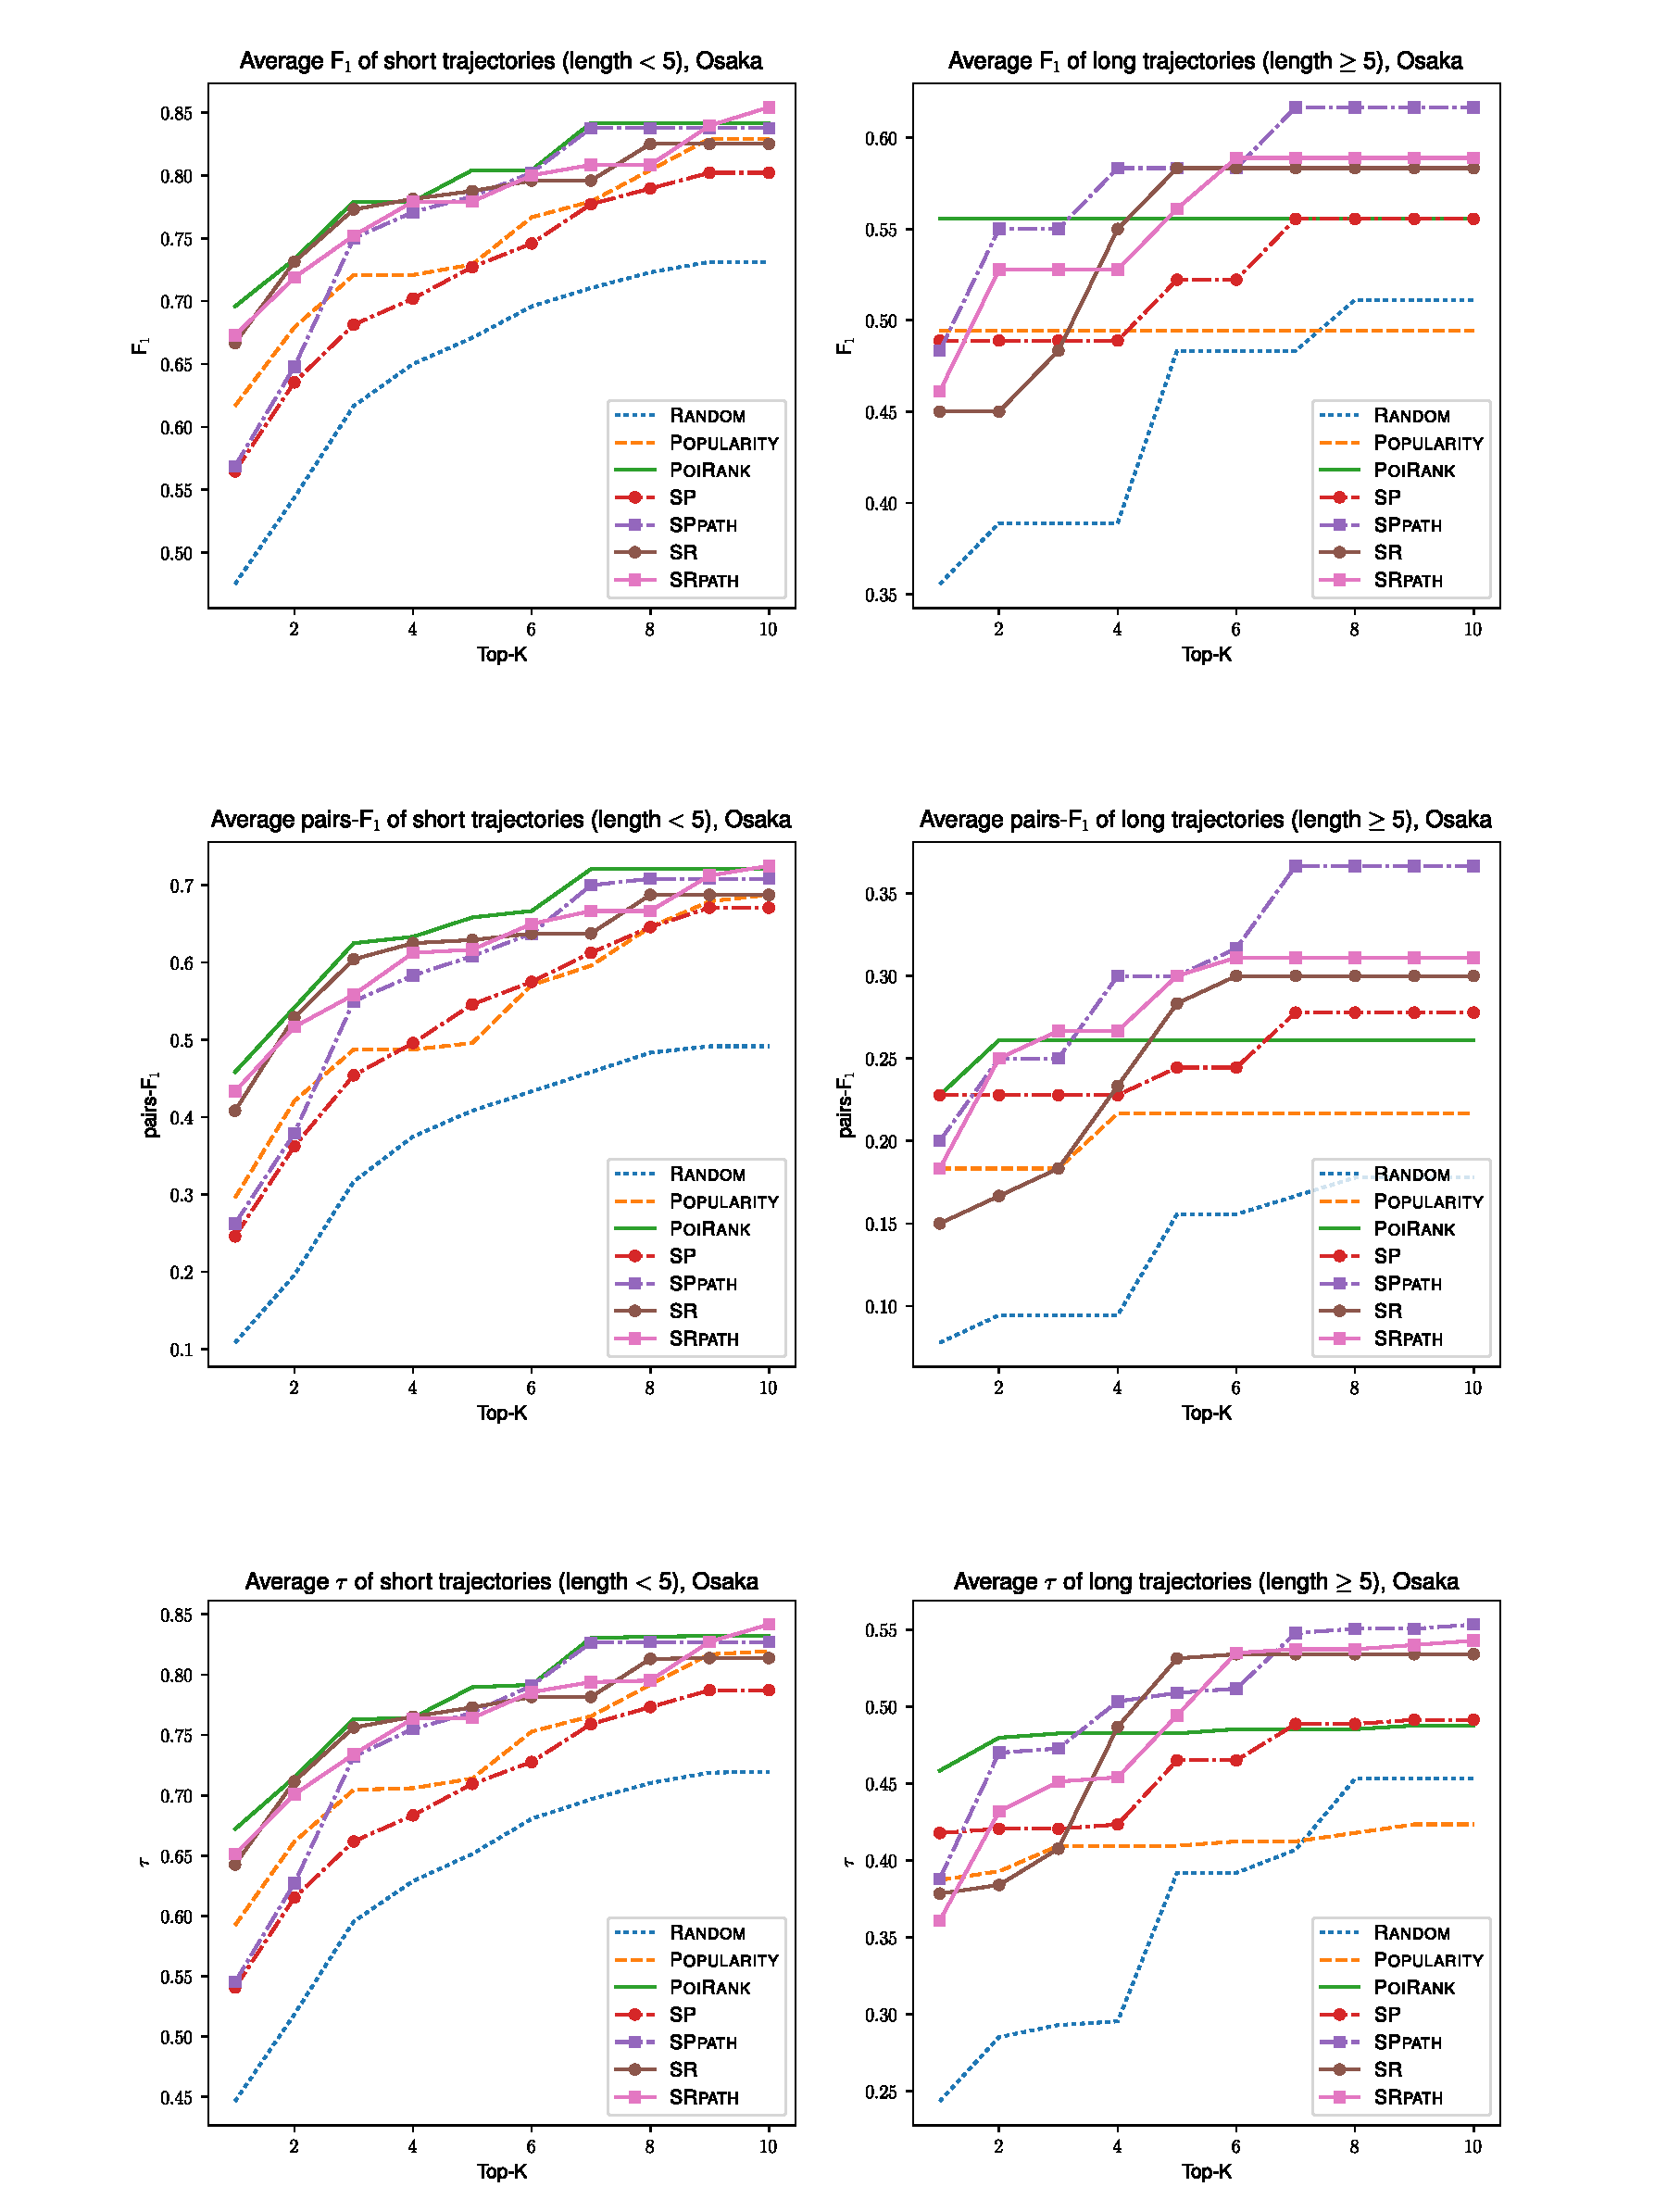
\includepdf[pages={1-}]{plot_topk.pdf}


\end{document}
